\documentclass[11pt,a4paper,headinclude,footinclude,DIV16]{scrreprt}
\usepackage[usenames,dvipsnames,table]{xcolor} % include at beginning because of compitibility issues
\usepackage[english]{babel}
\usepackage[utf8]{inputenc}
\usepackage[automark]{scrpage2}
\usepackage[normalem]{ulem}
\usepackage{amsmath}
\usepackage{amsfonts}
\usepackage{amssymb}
\usepackage{booktabs}
\usepackage{enumerate}
\usepackage{hyperref}
\usepackage{graphicx}
\usepackage{listings}
\usepackage{makeidx}
\usepackage[square,numbers]{natbib}
\usepackage{pdflscape}
\usepackage{rotating}
\usepackage{subfig}
\usepackage{tabularx}
\usepackage{theorem}
\usepackage{tikz}
\usepackage{tikz-qtree}
\usepackage{units}
\usepackage{url}
\usepackage{xspace}
\usepackage{accsupp}
\hypersetup{bookmarksdepth=3}
\usetikzlibrary{arrows}
\usetikzlibrary{backgrounds}
\usetikzlibrary{decorations.pathmorphing}
\usetikzlibrary{fit}
\usetikzlibrary{patterns}
\usetikzlibrary{positioning}
\usetikzlibrary{shapes}
\usetikzlibrary{trees}
\newcommand{\textcolordummy}[2]{#2}
\newcommand{\textcolordigits}{\textcolor{Mulberry}}
\lstset{showstringspaces=false,
 inputencoding=ansinew,
 breaklines=true,
 tabsize=4,
 columns=flexible,
 literate={0}{{\textcolordigits{0}}}{1}%
          {1}{{\textcolordigits{1}}}{1}%
          {2}{{\textcolordigits{2}}}{1}%
          {3}{{\textcolordigits{3}}}{1}%
          {4}{{\textcolordigits{4}}}{1}%
          {5}{{\textcolordigits{5}}}{1}%
          {6}{{\textcolordigits{6}}}{1}%
          {7}{{\textcolordigits{7}}}{1}%
          {8}{{\textcolordigits{8}}}{1}%
          {9}{{\textcolordigits{9}}}{1}%
          {.0}{{\textcolordigits{.0}}}{2}% Following is to ensure that only periods
          {.1}{{\textcolordigits{.1}}}{2}% followed by a digit are changed.
          {.2}{{\textcolordigits{.2}}}{2}%
          {.3}{{\textcolordigits{.3}}}{2}%
          {.4}{{\textcolordigits{.4}}}{2}%
          {.5}{{\textcolordigits{.5}}}{2}%
          {.6}{{\textcolordigits{.6}}}{2}%
          {.7}{{\textcolordigits{.7}}}{2}%
          {.8}{{\textcolordigits{.8}}}{2}%
          {.9}{{\textcolordigits{.9}}}{2}%
          {e0}{{\textcolordigits{e0}}}{2}% Following is to ensure that only periods
          {e1}{{\textcolordigits{e1}}}{2}% followed by a digit are changed.
          {e2}{{\textcolordigits{e2}}}{2}%
          {e3}{{\textcolordigits{e3}}}{2}%
          {e4}{{\textcolordigits{e4}}}{2}%
          {e5}{{\textcolordigits{e5}}}{2}%
          {e6}{{\textcolordigits{e6}}}{2}%
          {e7}{{\textcolordigits{e7}}}{2}%
          {e8}{{\textcolordigits{e8}}}{2}%
          {e9}{{\textcolordigits{e9}}}{2}%
          {e-0}{{\textcolordigits{e-0}}}{2}% Following is to ensure that only periods
          {e-1}{{\textcolordigits{e-1}}}{2}% followed by a digit are changed.
          {e-2}{{\textcolordigits{e-2}}}{2}%
          {e-3}{{\textcolordigits{e-3}}}{2}%
          {e-4}{{\textcolordigits{e-4}}}{2}%
          {e-5}{{\textcolordigits{e-5}}}{2}%
          {e-6}{{\textcolordigits{e-6}}}{2}%
          {e-7}{{\textcolordigits{e-7}}}{2}%
          {e-8}{{\textcolordigits{e-8}}}{2}%
          {e-9}{{\textcolordigits{e-9}}}{2},
}

% for listings of bash code
\lstdefinestyle{Bash}{
 language=Bash,
 backgroundcolor=\color{lightgray},
 basicstyle=\ttfamily\small\let\textcolor\textcolordummy,
 numbers=none,
 captionpos=b,
 tabsize=4,
 frame=single,
 rulecolor=\color{lightgray},
 framerule=1pt,
 framesep=1pt,
 rulesep=0pt,
 aboveskip=\bigskipamount,
 belowskip=\bigskipamount
}

% for listings of shell code
\lstdefinestyle{Shell}{
 language=sh,
 numbers=left,
 numbersep=5pt,
 numberstyle=\tiny\noncopynumber,
 basicstyle=\ttfamily\scriptsize,
 stringstyle=\color{BrickRed}\ttfamily\let\textcolor\textcolordummy,
 commentstyle=\color[gray]{0.35}\ttfamily\itshape\let\textcolor\textcolordummy,
}

% for listings of DuMuX code
\lstdefinestyle{DumuxCode}{
  language=C++,
  extendedchars=true,
  escapeinside={/*@}{@*/}, % escape the long comments
  numbers=left,
  numbersep=5pt,
  numberstyle=\tiny\noncopynumber,
  basicstyle=\ttfamily\scriptsize,
  keywordstyle=\color{dumuxBlue}\ttfamily\let\textcolor\textcolordummy,
  stringstyle=\color{BrickRed}\ttfamily\let\textcolor\textcolordummy,
  commentstyle=\color[gray]{0.35}\ttfamily\itshape\let\textcolor\textcolordummy,
  emph={NEW_TYPE_TAG, NEW_PROP_TAG, UNSET_PROP, TTAG, PTAG,
       SET_PROP, GET_PROP, GET_PROP_VALUE, GET_PROP_TYPE,
       SET_BOOL_PROP, SET_STRING_PROP, SET_SCALAR_PROP, SET_TYPE_PROP, SET_INT_PROP,
       GET_BOOL_PROP, GET_STRING_PROP, GET_SCALAR_PROP, GET_TYPE_PROP, GET_INT_PROP,
       GET_PARAM, GET_PARAM_FROM_GROUP, GET_RUNTIME_PARAM, GET_RUNTIME_PARAM_FROM_GROUP},
  emphstyle=\color{OliveGreen}\let\textcolor\textcolordummy,
  directivestyle=\color{Brown}\ttfamily\let\textcolor\textcolordummy,
}

% for listings of DuMuX parameter files
\lstdefinestyle{DumuxParameterFile}{
 language=sh,
 numbers=left,
 numbersep=5pt,
 numberstyle=\tiny\noncopynumber,
 basicstyle=\ttfamily\scriptsize,
 stringstyle=\color{BrickRed}\ttfamily\let\textcolor\textcolordummy,
 commentstyle=\color[gray]{0.35}\ttfamily\itshape\let\textcolor\textcolordummy,
 morecomment=[l][\color{dumuxBlue}\let\textcolor\textcolordummy]{[},
}

\newcommand{\noncopynumber}[1]{
    \BeginAccSupp{method=escape,ActualText={}}
    #1
    \EndAccSupp{}
}


\DeclareGraphicsExtensions{.pdf, .jpg}

% Dune and Dumux logo
\newcommand{\Dune}{{DUNE}\xspace}
\newcommand{\Dumux}{\texorpdfstring{Du\-Mu$^\text{x}$\xspace}{DuMuX\xspace}}
\newcommand{\DumuxVersion}{3.0}
\definecolor{dumuxYellow}{HTML}{E19417}
\definecolor{dumuxBlue}{HTML}{0C73CF}

% sytles
\newcommand{\nextline}{\par\phantom{a}\vspace*{0.1\textwidth}}
\newcommand{\snakeline}{\uwave{\mbox{}}}
\DeclareRobustCommand\Cplusplus{\texorpdfstring{C\nolinebreak[4]\hspace{-.05em}\raisebox{.4ex}{\tiny\bfseries ++}\xspace}{C++}}

% notation
\newcommand{\porosity}{\phi}
\newcommand{\saturation}{S}

% a new counter you can give a label to it and thus reference it
% syntax: \numberThis{printedTextToBeLabeled}{label}
% if you wanted a \newline after a numbered thing, you could just add a empty line after ``\label{#2}''
\newcounter{thingCounter}
\renewcommand{\thethingCounter}{\arabic{thingCounter}}
\newcommand{\numberThis}[2]{%
        \refstepcounter{thingCounter}%
        \thethingCounter.\ #1 \label{#2}
}

%The theorems
\theorembodyfont{\upshape}
\theoremheaderfont{\sffamily\bfseries}
\newtheorem{lst}{Listing}

\DeclareMathOperator{\grad}{\mathbf{grad}}
\DeclareMathOperator{\curl}{curl}
\DeclareMathOperator{\Div}{div}

\pagestyle{scrheadings}

\title{
\begin{center}

\includegraphics[width=0.7\textwidth]{../logo/dumux_logo_hires_whitebg.png}
\\[3cm]
{\Huge Handbook}
\end{center}
}

\author{}

\date{Version \DumuxVersion}

\publishers{%
\vspace{10mm}
{\normalsize Lehrstuhl f\"ur Hydromechanik und Hydrosystemmodellierung, \\
Universit\"at Stuttgart, Paffenwaldring 61, D-70569 Stuttgart, Germany}\\
%
\bigskip
{\normalsize \texttt{\url{http://dumux.org}}}\\
}

\makeindex

\begin{document}

\maketitle

\setcounter{tocdepth}{1}
\tableofcontents
\newpage

\chapter{Introduction}
\Dumux aims to be a generic framework for the simulation of multiphase
fluid flow and transport processes in porous media using continuum
mechanical approaches.  At the same time, \Dumux aims to deliver
top-notch computational performance, high flexibility, a sound
software architecture and the ability to run on anything from single
processor systems to highly parallel supercomputers with specialized
hardware architectures.

The means to achieve these somewhat contradictory goals are the
thorough use of object-oriented design in conjunction with template
programming. These requirements call for \Cplusplus as the implementation
language.

One of the more complex issues when dealing with parallel continuum
models is managing the grids used for the spatial discretization of
the physical model. To date, no generic and efficient approach exists
for all possible cases, so \Dumux is build on top of \Dune, the
\textbf{D}istributed and \textbf{U}nified \textbf{N}umerics
\textbf{E}nvironment~\cite{DUNE-HP}. \Dune provides a generic interface
to many existing grid management libraries such as UG~\cite{UG-HP},
ALUGrid~\cite{ALUGRID-HP,alugrid2016} and a few more.
DUNE also extensively uses template programming in order to
achieve minimal overhead when accessing the underlying grid
libraries\footnote{In fact, the performance penalty resulting from the
use of \Dune's grid interface is usually negligible~\cite{BURRI2006}.}.
\begin{figure}[hbt]
  \centering
  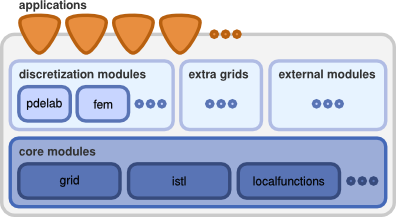
\includegraphics[width=.5\linewidth, keepaspectratio]{png/dunedesign.png}
  \caption{
    \label{fig:dune-design}
    A high-level overview of \Dune's design is available on the project's
    web site~\cite{DUNE-HP}.
  }
\end{figure}

DUNE's grid interface is independent of the spatial dimension of the
underlying grid. For this purpose, it uses the concept of
co-dimensional entities. Roughly speaking, an entity of co-dimension
$0$ constitutes a cell, co-dimension $1$ entities are faces between
cells, co-dimension $2$ are edges, and so on until co-dimension $n$
which are the cell's vertices.  The \Dune grid interface generally
assumes that all entities are convex polytopes, which means that it
must be possible to express each entity as the convex hull of a set of
vertices. For the sake of efficiency, all entities are further expressed in terms
of so-called reference elements which are transformed to the actual
spatial incarnation within the grid by a so-called geometry
function. Here, a reference element for an
entity can be thought of as a prototype for the actual grid
entity. For example, if we used a grid which applied hexahedrons as cells,
the reference element for each cell would be the unit cube $[0, 1]^3$
and the geometry function would scale and translate the cube so that
it matches the grid's cell. A quick overview of reference elements and the
related numbering can be obtained from the DUNE cheat sheet
(\url{https://www.dune-project.org/pdf/dune-cheat-sheet.pdf}).
For a more thorough description of \Dune's
grid definition, see~\cite{BASTIAN2008}.

In addition to the grid interface, \Dune also provides quite a few
additional modules, of which the \texttt{dune-localfunctions} and
\texttt{dune-istl} modules are the most relevant in the context of
this handbook. \texttt{dune-localfunctions} provides a set of generic
finite element shape functions, while \texttt{dune-istl} is the
\textbf{I}terative \textbf{S}olver \textbf{T}emplate \textbf{L}ibrary
and provides generic, highly optimized linear algebra routines for
solving the generated systems.

\Dumux comes in form of an additional module \texttt{dumux}.
It depends on the \Dune core modules
\texttt{dune-common}, \texttt{dune-grid}, \texttt{dune-istl}, and \texttt{dune-localfunctions}.
The main intention of \Dumux is to provide a framework for an easy and efficient
implementation of new physical models for porous media flow problems,
ranging from problem formulation and the selection of
spatial and temporal discretization schemes as well as nonlinear solvers,
to general concepts for model coupling.
Moreover, \Dumux includes ready to use numerical models and a few example applications.

This is the handbook to a new minor version update of \Dumux: version 3.1.
The release contains improvements and new features compared to the 3.0 version.
The update is  backwards compatible with the last release 3.0.
To facilitate the transition for our users, we have created a changelog
helping to update programs from version 3.0 to version 3.1, and giving an overview over new capabilities.
It is available online:
\url{https://git.iws.uni-stuttgart.de/dumux-repositories/dumux/blob/master/CHANGELOG.md}.
We highly recommend all our users to transition with us to the most recent version of \Dumux
and wish everyone a brand-new and exciting simulation experience.


\chapter{Getting started}
In this chapter we provide a quick start guide to
your first \Dumux experience.
The first section contains instructions on how to very quickly install \Dumux.
More detailed information on how to obtain source code, build and test \Dune and \Dumux
follows in the second section of this chapter. The second section also contains information on
how to build the documentation and about external libraries and modules.
\section{Prerequisites} \label{sec:prerequisites}
For this quick start guide the following software packages are required:
\begin{itemize}
\item GitLab client
\item A standard compliant C++ compiler supporting C++11 and the C++14 feature set of GCC 4.9. We support GCC 4.9 or newer and Clang 3.8 or newer.
\item CMake 2.8.12 or newer
\item pkg-config
\item ParaView (to visualize the results)
\end{itemize}

\section{Obtaining code and configuring all modules with a script}
We provide you with a shell-script \texttt{installDumux.sh} that facilitates setting up a {\Dune}/{\Dumux} directory tree
and configures all modules with CMake.
Copy the following lines into a text file named \texttt{installDumux.sh}:
\lstinputlisting[style=DumuxCode, numbersep=5pt, firstline=1, firstnumber=1]{installDumux.sh}

Place the \texttt{installDumux.sh} script in the directory where you want to install \Dumux and \Dune (a single
root folder \texttt{DUMUX} will be produced, so you do not need to provide one). Make \texttt{installDumux.sh} executable and run the script by typing into the terminal: \texttt{./installDumux.sh}

Configuring \Dune and \Dumux is done by the command-line script \texttt{dunecontrol}
using optimized configure options, see the line entitled \texttt{\# run build} in the \texttt{installDumux.sh} script.
More details about the build-system can be found in section \ref{buildIt}.

\subsection{A first test run of \Dumux}
When the \texttt{installDumux.sh} script from the subsection above has run successfully, you can execute a second script that
will compile and run a simple one-phase ground water flow example and will visualize the result using ParaView.
The test script can be obtained by copying the following lines into a text file named \texttt{test\_dumux.sh}
that has to be located in the same directory as the installation script.
\begin{lstlisting}[style=DumuxCode]
cd DUMUX/dumux/build-cmake/test/porousmediumflow/1p/implicit/isothermal
make -B test_1p_tpfa
./test_1p_tpfa params.input
paraview *pvd
\end{lstlisting}
After making \texttt{test\_dumux.sh} executable, it can be executed by typing into the terminal: \texttt{./test\_dumux.sh}.
If everything works fine, a ParaView window with the result should open automatically, showing the initial
conditions. Advance ParaView to the next frame (green arrow button) and rescale to data range (green double arrow on top right) to admire
the colorful pressure distribution.

% \section{Detailed Installation Instructions}
% \label{install}

Installing \Dumux means that you first unpack \Dune and \Dumux in a root directory,
(section \ref{sc:ObtainingSourceCode}).
In a second step of the installation, all modules are configured with CMake
(section \ref{buildIt}).
After successfull installation of \Dumux we guide you to start a test application,
described in section \ref{quick-start-guide}.
In section \ref{sec:build-doxy-doc} we explain how to build the \Dumux documentation.
Lastly, section \ref{sec:external-modules-libraries} provides details on optional libraries and modules.

In a technical sense \Dumux is a module of \Dune.
Thus, the installation procedure of \Dumux is the same as that of \Dune.
Details regarding the installation of \Dune are provided on the \Dune website \cite{DUNE-HP}.


\section{Obtaining Source Code for \Dune and \Dumux}
\label{sc:ObtainingSourceCode}
The \Dumux release and trunk (developer tree) are based on the most recent
\Dune release 2.6, comprising the core modules dune-common, dune-geometry, dune-grid,
dune-istl and dune-localfunctions. For working with \Dumux, these modules are required.
All \Dune modules, including the \Dumux module, get extracted into a common root directory, as it
is done in an ordinary \Dune installation.
We usually name our root directory \texttt{DUMUX} but an arbitrary name can be chosen.
Source code files for each \Dune module are contained in their own subdirectory within the root directory.
The subdirectories for the modules are named after the module names (depending on how
the modules were obtained a version number is added to the module name).
The name of each \Dune module is defined in the file \texttt{dune.module}, which is
in the root directory of the respective module. This should not be changed by the user.

Two possibilities exist to get the source code of \Dune and \Dumux.
Firstly, \Dune and \Dumux can be downloaded as tar files from the respective \Dune and \Dumux website.
They have to be extracted as described in the next paragraph.
% % TODO: alpha version was not released with a tarball. For the next releases the following lines need to be deleted again
% There is no tar file for the current \DumuxVersion~release.
% Secondly, a method to obtain the most recent source code (or, more generally, any of its previous revisions) by direct access
% to the software repositories of the revision control system is described in the subsequent part.
% Be aware that you cannot get \texttt{dumux-devel} or the external libraries from \texttt{dumux-external} unless
% you have an GitLab account with the right privileges.

In section \ref{sec:prerequisites} we list some prerequisites for running \Dune and \Dumux.
Please check in said paragraph whether you can fulfill them before continuing.

% TODO: alpha version was not released with a tarball. For the next releases the following lines need to be uncommented again
\paragraph{Obtaining the software by installing tar files}
The slightly old-fashionedly named tape-archive-file, shortly named tar file or
tarball, is a common file format for distributing collections of files contained
within these archives.
The extraction from the tar files is done as follows:
Download the tarballs from the respective \Dune (version 2.6) and \Dumux websites
to a certain folder in your file system.
Create the common root directory, named \texttt{DUMUX} in the example below.
Then extract the content of the tar files, e.\,g. with the command-line program
\texttt{tar}.
This can be achieved by the following shell commands. Replace \texttt{path\_to\_tarball}
with the directory name where the downloaded files are actually located.
After extraction, the actual name of the dumux subdirectory is \texttt{dumux-\DumuxVersion}
(or whatever version you downloaded).

\begin{lstlisting}[style=Bash]
$ mkdir DUMUX
$ cd DUMUX
$ tar xzvf path_to_tarball_of/dune-common-2.6.0.tar.gz
$ tar xzvf path_to_tarball_of/dune-geometry-2.6.0.tar.gz
$ tar xzvf path_to_tarball_of/dune-grid-2.6.0.tar.gz
$ tar xzvf path_to_tarball_of/dune-istl-2.6.0.tar.gz
$ tar xzvf path_to_tarball_of/dune-localfunctions-2.6.0.tar.gz
$ tar xzvf path_to_tarball_of/dumux-3.0.tar.gz
\end{lstlisting}

Furthermore, if you wish to install the optional \Dune Grid-Howto which provides a tutorial
on the Dune grid interface, act similar.

\paragraph{Obtaining \Dune and \Dumux from software repositories}
Direct access to a software revision control system for downloading code can be of advantage later on.
It is easier to keep up with code changes and to receive important bug fixes.
\Dune and \Dumux use Git for their software repositories. To access them a Git client is needed.

In the technical language of Git, \emph{cloning a certain software version} means nothing more then fetching
a local copy from the software repository and laying it out in the file system.
In addition to the software, some more files for the use of the software revision
control system itself are created. If you have developer access to \Dumux, it is
also possible to do the opposite, i.\,e. to load up a modified revision of software
into the software repository. This is usually termed as \emph{commit} and \emph{push}.

The installation procedure is done as follows:
Create a common root directory, named e.g. \texttt{DUMUX} in the lines below.
Then, enter the previously created directory and check out the desired modules.
As you see below, the check-out uses two different servers for getting the sources,
one for \Dune and one for \Dumux.

\begin{lstlisting}[style=Bash]
$ mkdir DUMUX
$ cd DUMUX
$ git clone -b releases/2.6 https://gitlab.dune-project.org/core/dune-common.git
$ git clone -b releases/2.6 https://gitlab.dune-project.org/core/dune-geometry.git
$ git clone -b releases/2.6 https://gitlab.dune-project.org/core/dune-grid.git
$ git clone -b releases/2.6 https://gitlab.dune-project.org/core/dune-istl.git
$ git clone -b releases/2.6 https://gitlab.dune-project.org/core/dune-localfunctions.git
$ git clone -b releases/3.0 https://git.iws.uni-stuttgart.de/dumux-repositories/dumux.git
\end{lstlisting}

The newest and maybe unstable developments of \Dune and \Dumux are also provided in these repositories and can be found in the \emph{master} branch.
Please check the \Dune website \cite{DUNE-HP} for further information on the \Dune development. We always try to keep up with the latest developments of \Dune.
However, the current \Dumux release is based on the stable 2.6 release and it might not compile without further adaptations using the newest versions of \Dune.

Furthermore, if you wish to install the optional \Dune Grid-Howto which provides a tutorial
on the Dune grid interface, act similar.

%TODO:currently, no DUNE patches necessary! Uncomment this section in case this changes again in the future.
%
% \paragraph{Patching \Dune or external libraries}
% \label{sc:patchingDUNE}
% Patching of \Dune modules in order to work together with \Dumux can be necessary for several reasons.
% Software like a compiler or even a standard library
% changes at times. But, for example, a certain release of a software component that we depend on,
% may not reflect that change and thus it has to be modified.
% In the dynamic developing process of software which depends on other modules it is not always feasible
% to adapt everything to the most recent version of each module. They may fix problems with a certain module
% of a certain release without introducing too much structural change.
%
% \Dumux contains patches and documentation about their usage and application within the
% directory \texttt{dumux/patches}.
% Please check the README file in that directory for recent information.
% In general, a patch can be applied as follows
% (the exact command or the used parameters may be slightly different).
% We include here an example of a patching dune-grid.
%
% \begin{lstlisting}[style=Bash]
% $ # make sure you are in the common root directory
% $ cd dune-grid
% $ patch -p0 < ../dumux/patches/grid-2.3.1.patch
% \end{lstlisting}
%
% It can be removed by
% \begin{lstlisting}[style=Bash]
% $ path -p0 -R < ../dumux/patches/grid-2.3.1.patch
% \end{lstlisting}

\paragraph{Hints for \Dumux-Developers}
If you also want to actively participate in the development of \Dumux, you can allways send patches
to the Mailing list.
To get more involved, you can apply either for full developer
access or for developer access on certain parts of \Dumux. Granted developer access means that
you are allowed to commit own code and that you can access the \texttt{dumux-devel} module.
This enhances \texttt{dumux} by providing maybe unstable code from the developer group.

\section{Build of \Dune and \Dumux}
\label{buildIt}
Configuring \Dune and \Dumux is done by the shell-command \texttt{dunecontrol} which is part of the \Dune build system.
If you are interested in more details about the build system that is used,
they can be found in the \Dune buildsystem documentation\footnote{\url{https://www.dune-project.org/buildsystem/}} and
CMake's documentation\footnote{\url{https://cmake.org/documentation/}}.
If something fails during the execution of \texttt{dunecontrol} feel free to report it to the \Dune or \Dumux developer mailing list,
but please include error details.

It is possible to compile \Dumux with nearly no explicit options to the build system.
However, for the successful compilation of \Dune and \Dumux, it is currently necessary to pass
the option \texttt{-fno-strict-aliasing} to the \Cplusplus compiler,
which is done here via a command-line argument to \texttt{dunecontrol}:
\begin{lstlisting}[style=Bash]
$ # make sure you are in the common root directory
$ ./dune-common/bin/dunecontrol --configure-opts="CXXFLAGS=-fno-strict-aliasing" --use-cmake all
\end{lstlisting}

Too many options can make life hard. That's why usually option files are being used together with \texttt{dunecontrol} and its sub-tools.
Larger sets of options are kept in them. If you are going to compile with options suited for debugging the code, the following
can be a starting point:
\begin{lstlisting}[style=Bash]
$ # make sure you are in the common root directory
$ cp dumux/debug.opts my-debug.opts      # create a personal version
$ gedit my-debug.opts                    # optional editing the options file
$ ./dune-common/bin/dunecontrol --opts=my-debug.opts --use-cmake all
\end{lstlisting}

More optimized code, which is typically not usable for standard debugging tasks, can be produced by
\begin{lstlisting}[style=Bash]
$ cp dumux/optim.opts my-optim.opts
$ ./dune-common/bin/dunecontrol --opts=my-optim.opts --use-cmake all
\end{lstlisting}

Sometimes, it is necessary to have additional options which
are specific to a package set of an operating system or
sometimes you have your own preferences.
Feel free to work with your own set of options, which may evolve over time.
The option files above are to be understood more as a starting point
for setting up an own customization than as something which is fixed.
The use of external libraries can make it necessary to add quite many options in an option file.
It can be helpful to give your customized option file its own name, as done above,
to avoid confusing it with the option files which came out of the distribution.

\section{The First Run of a Test Application}
\label{quick-start-guide}
The previous section showed how to install and compile \Dumux. This section
shall give a very brief introduction how to run a first test application and how
to visualize the first output files.\\
All executables are compiled in the \texttt{build} subdirectories of \Dumux.
If not given differently in the input files, this is \texttt{build-cmake} as default.

\begin{enumerate}
\item Go to the directory \texttt{build-cmake/test}. There, various test application
      folders can be found. Let us consider as example\\
      \texttt{porousmediumflow/2p/implicit/incompressible/test{\_}2p{\_}incompressible{\_}tpfa}.
\item Enter the folder \texttt{porousmediumflow/2p/implicit/incompressible}.\\ Type \texttt{make test{\_}2p{\_}incompressible{\_}tpfa}
      in order to compile the application\\ \texttt{test{\_}2p{\_}incompressible{\_}tpfa}. To run the simulation,
      type \texttt{./test{\_}2p{\_}incompressible{\_}tpfa params.input}
      into the console.
      The added \texttt{params.input} specifies that all
      important run-time parameters (like first timestep size, end of simulation and location
      of the grid file) can be found in a text file in the same directory  with the
      name \texttt{params.input}.
\item The simulation starts and produces some .vtu output files and also a .pvd
      file. The .pvd file can be used to examine time series and summarizes the .vtu
      files. It is possible to stop a running application by pressing $<$Ctrl$><$c$>$.
\item You can display the results using the visualization tool ParaView (or
      alternatively VisIt). Just type \texttt{paraview} in the console and open the
      .pvd file. On the left hand side, you can choose the desired parameter to be displayed.
\end{enumerate}

\section{Building Documentation}

The building of included documentation like this handbook requires \LaTeX{} and auxiliary tools
\texttt{bibtex}. One usually chooses a \LaTeX{} distribution like \texttt{texlive} for this purpose.
It is possible to switch off the building of the documentation by setting the switch \texttt{--disable-documentation}
in the \texttt{CONFIGURE\_FLAGS} of the building options, see section \ref{buildIt}.

\subsection{Doxygen}
\label{sec:build-doxy-doc}
Doxygen documentation is done by especially formatted comments integrated in the source code,
which can get extracted by the program \texttt{doxygen}. Beside extracting these comments,
\texttt{doxygen} builds up a web-browsable code structure documentation
like class hierarchy of code displayed as graphs, see \url{http://www.stack.nl/~dimitri/doxygen/}.

The Doxygen documentation of a module can be built, if \texttt{doxygen} is installed,
by running \texttt{dunecontrol}, entering the \texttt{build-*}directory, and execute
\texttt{make doc}. Then point your web browser to the file
\texttt{MODULE\_BUILD\_DIRECTORY/doc/doxygen/html/index.html} to read the generated documentation.
This should also work for other \Dune modules.

\subsection{Handbook}
To build the \Dumux handbook go into the \texttt{build-}directory and
run \texttt{make doc} or \texttt{make 0\_dumux-handbook\_pdf}. The pdf can then be found
in \texttt{MODULE\_BUILD\_DIRECTORY/doc/handbook/0\_dumux-handbook.pdf}.

\section{External Libraries and Modules} \label{sec:external-modules-libraries}
The libraries described below provide additional functionality but are not generally required to run \Dumux.
If you are going to use an external library check the information provided on the \Dune website%
\footnote{DUNE: External libraries, \url{https://www.dune-project.org/doc/external-libraries/}}.
If you are going to use an external \Dune module the website on external modules%
\footnote{DUNE: External modules, \url{https://www.dune-project.org/groups/external/}}
can be helpful.

Installing an external library can require additional libraries which are also used by \Dune.
For some libraries, such as BLAS or MPI, multiple versions can be installed on the system.
Make sure that it uses the same library as \Dune when configuring the external library.

Some of the libraries are then compiled within that directory and are not installed in
a different place, but \Dune may need to know their location. Thus, one may have to refer to
them as options for \texttt{dunecontrol}, for example via the options file \texttt{my-debug.opts}.
Make sure you compile the required external libraries before you run \texttt{dunecontrol}.

An easy way to install some of the libraries and modules given below is the
\texttt{installexternal.sh} script located in \texttt{bin}. The script
has to be called from your common root directory.


\subsection{List of External Libraries and Modules}
In the following list, you can find some external modules and external libraries,
and some more libraries and tools which are prerequisites for their use.

\begin{itemize}
\item \textbf{dune-ALUGrid}: Grid library, comes as a \Dune module.
  The parallel version needs also a graph partitioner, such as {ParMETIS}.
  Download: \url{https://gitlab.dune-project.org/extensions/dune-alugrid}

\item \textbf{dune-foamgrid}: External grid module. One- and two-dimensional grids
  in a physical space of arbitrary dimension; non-manifold grids, growth, element
  paramterizations, and movable vertices. This makes FoamGrid the grid data structure
  of choice for simulating structures such as foams, discrete fracture networks,
  or network flow problems.
  Download: \url{https://gitlab.dune-project.org/extensions/dune-foamgrid}
  
\item \textbf{opm-grid}: opm-grid is a DUNE module supporting grids in a corner-point format.
  Download: \url{https://github.com/OPM/opm-grid.git}
  
\item \textbf{dune-subgrid}: The dune-subgrid module is a meta-grid implementation that allows 
to mark elements of another hierarchical dune grid and use this sub-grid just like a regular grid.
The set of marked elements can then be accessed as a hierarchical dune grid in its own right.
Dune-Subgrid provides the full grid interface including adaptive mesh refinement.
  Download: \url{https://git.imp.fu-berlin.de/agnumpde/dune-subgrid.git}
  
\item \textbf{dune-spgrid}: The DUNE module dune-spgrid provides a structured, parallel grid
and supports periodic boundary conditions.
  Download: \url{https://gitlab.dune-project.org/extensions/dune-spgrid.git}

\item \textbf{SuperLU}: External library for solving linear equations. SuperLU is a general purpose
  library for the direct solution of large, sparse, non-symmetric systems of linear equations.
  Download: \url{http://crd.lbl.gov/~xiaoye/SuperLU}

\item \textbf{UMFPack}: External library for solving linear equeations. It is part of SuiteSparse.

\item \textbf{dune-UG}: External library for use as grid. UG is a toolbox for unstructured grids, released under GPL.
  To build UG the tools \texttt{lex}/\texttt{yacc} or the GNU variants of \texttt{flex}/\texttt{bison} must be provided.
  Download: \url{https://gitlab.dune-project.org/staging/dune-uggrid}
\end{itemize}

The following are dependencies of some of the used libraries. You will need them
depending on which modules of \Dune and which external libraries you use.

\begin{itemize}
\item \textbf{MPI}: The parallel version of \Dune and also some of the external dependencies need MPI
  when they are going to be built for parallel computing. \texttt{OpenMPI} and \texttt{MPICH} in a recent
  version have been reported to work.

\item \textbf{BLAS}: SuperLU makes use of BLAS. Thus install GotoBLAS2, ATLAS, non-optimized BLAS
  or BLAS provided by a chip manufacturer. Take care that the installation scripts select the intended
  version of BLAS.

\item \textbf{METIS} and \textbf{ParMETIS}: This are dependencies of ALUGrid and can be used with UG, if run in parallel.

\item \textbf{Compilers}: Beside \texttt{g++}, \Dune can be built with Clang from the LLVM project and
  Intel \Cplusplus compiler. C and Fortran compilers are needed for some external libraries. As code of
  different compilers is linked together they have to be be compatible with each other.
\end{itemize}


\chapter{Tutorial}\label{chp:tutorial}
Decription of new tutorial is going to come soon!

\section{Further Practice}
\label{tutorial-furtherpractice}

If there is a need for further practice, we refer here to the test problems that
are already implemented in \Dumux. Several examples for all models
can be found in the \texttt{test}-directory. An overview over the available test
cases can be found in the class documentation \url{http://www.dumux.org/documentation.php}.
There you also find a \emph{feature-list} for the individual tests.%TODO

Another possibility to gain more experience with \Dumux is the \texttt{dumux-lecture} module
that contains different application examples that are used in the lectures at the 
Department of Hydromechanics and Modelling of Hydrosystems in Stuttgart.
The \texttt{dumux-lecture} module can be obtained as follows:
\begin{lstlisting}[style=Bash]
$ git clone https://git.iws.uni-stuttgart.de/dumux-repositories/dumux-lecture.git
\end{lstlisting}
The module is structured based on the different lectures: 
\begin{itemize}
\item mm: Multiphase Modelling,
\item efm: Environmental Fluid Mechanics,
\item mhs: Modelling of Hydrosystems.
\end{itemize}
The majority of applications is covered in the course Multiphase Modelling (mm), 
while there are also some basic examples from the
courses Environmental Fluid Mechanics (efm) and Modelling of Hydrosystems (mhs). 
These applications are primarily designed to enhance the understanding of conceptualizing the
governing physical processes and their implementation in a numerical simulator. 
Different aspects of modelling multi-phase multi-component flow and transport processes are shown.
The lectures focus on questions like, e. g., the assignment of boundary conditions, the choice of the 
appropriate physics for a given problem (which phases, which components), discretization issues,
time stepping. You can find, e. g., a comparison of different two-phase flow problems: The
more simple approach considers two immiscible fluids while components in both phases with interphase
mass transfer are considered in the more complex approach.
All scenarios and their physical background are explained in additional .tex-files,
which are provided in sub-directories named \texttt{description}. The following test cases are 
contained in the \texttt{dumux-lecture} module:
\begin{itemize}
\item \texttt{buckleyleverett}: The Buckley-Leverett Problem is a classical porous media flow show case
\item \texttt{co2plume}: Analysis of the influence of the gravitational number on the $\text{CO}_2$ plume 
\item \texttt{columnxylene}: A VEGAS experiment
\item \texttt{convectivemixing}: A test case related to CO$_2$ storage
\item \texttt{fuelcell}%TODO
\item \texttt{heatpipe}: A show case for two-phase two-component flow with heat fluxes
\item \texttt{heavyoil}: Steam assisted gravity drainage (SAGD)
\item \texttt{henryproblem}: A show case related to salt water intrusion
\item \texttt{mcwhorter}: The McWhorter Problem is a classical porous media flow show case
\item \texttt{naplinfiltration}: Infiltration of non-aqueous phase liquid (NAPL) into soil
\item \texttt{remediationscenarios}: Test case for NAPL contaminated unsaturated soils
\item \texttt{groundwater}: Simple groundwater flow case for the course Modelling of Hydrosystems (mhs)
\item Different single/two-phase, single/two-component problems: Examples from the course Environmental Fluid Mechanics (efm)
\end{itemize}


\chapter{Overview and Infrastructure}
This chapter provides an overview of the general structure in \Dumux \ref{sc_structure}
and gives help for basic work with \Dumux
(\ref{sc_newfoldersetup},\ref{sc_parameterfiles},\ref{sc_restartsimulations}, \ref{sc_developingdumux}).
Further it presents useful external tools \ref{sc_externaltools} and basic
concepts \ref{sc_linearsystem}.
\section{Directory Structure}
\todo[inline]{Wollen wir hier alle Unterordner kurz vorstellen und \emph{kurz} erklären,
  was in deren Unterordnern zu finden ist?}
We briefly describe the directory structure of \Dumux in terms
of subdirectories, source files, and tests. For more details,
the Doxygen documentation should be considered.
\Dumux comes in form of a DUNE module \texttt{dumux}.
It has a similar structure as other DUNE modules like \texttt{dune-grid}.
The following subdirectories are within the module's root directory,
from now on assumed to be \texttt{/}:
\begin{itemize}
\item \texttt{bin}: contains binaries, e.g. used for the automatic testing
\item \texttt{CMake}: the configuration options
for building \Dumux using CMake. See the file \texttt{INSTALL.cmake} in
the root directory of \texttt{dumux} for details. Of course,
it is also possible to use the DUNE buildsystem just like for the other
DUNE modules.
\item \texttt{doc}: contains the Doxygen documentation in \texttt{doxygen},
this handbook in \texttt{handbook}, and the \Dumux logo in various formats in
\texttt{logo}. The html documentation produced by Doxygen can be accessed as usual,
namely, by opening \texttt{doc/doxygen/html/index.html} with a web browser.
\item \texttt{dumux}: the \Dumux source files. See Section \ref{sec:dumux} for details.
\item \texttt{test}: tests for each numerical model and the property system.
See Section \ref{sec:test} for details.
\item \texttt{tutorial}: contains the tutorials described in Chapter \ref{chp:tutorial}.
\end{itemize}


\subsection{The directory \texttt{dumux}}
\label{sec:dumux}

The directory \texttt{dumux} contains the \Dumux source files. It consists of the
following subdirectories (see Figure \ref{fig:dumux-structure}):

\begin{itemize}

\item \texttt{implicit}:
the general fully implicit method is contained in the subdirectory \texttt{common}.
The subdirectories \texttt{box} and \texttt{cellcentered} contain the code for the according
discretization types. They also contain files \texttt{..fvelementgeometry.hh} employed
by the box or cc method to extract the dual mesh geometry information out of the primal one.
Each of the other subdirectories contain a derived specific numerical model.
% The files \texttt{pdelabboxassembler.hh} and \texttt{pdelabboxlocaloperator.hh} allow the use of the DUNE module \texttt{dune-pdelab}.

\item \texttt{common}:
general stuff like the property system and the time management for the
fully coupled as well as the decoupled models,
% the interface for the Pardiso direct solver library \cite{Pardiso},
and the \texttt{start.hh} file that includes the common routine for starting a model called in the main function.

\item \texttt{decoupled}:
 numerical models to solve the pressure equation as part of the fractional flow
 formulation. The specific models are contained
 in corresponding subdirectories. In each model folder are subdirectories for the
 implicit pressure equation sorted by the employed discretization method, and for the
 explicit transport equation. The general decoupled formulation for the implicit
 pressure explicit transport formulation can be found in the subdirectory \texttt{common}.

% \item \texttt{fractionalflow}:
% the (non-compositional) fractional flow model, which utilizes the IMPES method
% contained in the subdirectory \texttt{impes}.

% \item \texttt{functions}:
% the Crouzeix--Raviart function implemented in the style of \texttt{dune-disc}'s P1 function.

% \item \texttt{fvgeometry}:
% employed by the box method to extract the dual mesh geometry information out of the
% primal one.

\item \texttt{io}: additional in-/output possibilities like restart files, gnuplot-interface
and a VTKWriter extension.

\item \texttt{material}: everything related to material parameters and
constitutive equations. The properties of a pure chemical substance (e.g. water) or
pseudo substance (e.g. air) can be found in the subdirectory \texttt{components}
with the base class \texttt{components/component.hh}. The fluidsytem in the folder
\texttt{fluidsystems} collects the information from the respective component and
binary coefficients files, and contains the fluid characteristics of phases
(e.g. viscosity, density, enthalpy, diffusion coefficients) for compositional or non-compositional multi-phase flow.

The base class for all spatially dependend variables -- like permeability and porosity  --
can be found in \texttt{spatialparams}. The base class in \texttt{implicitspatialparameters.hh}
also provides spatial averaging routines. All other spatial properties are specified in the specific
 files of the respective models. Furthermore, the constitutive relations --
 e.g. $p_c(S_w) $ -- are in \texttt{fluidmatrixinteractions},
while the necessary binary coefficients like the Henry coefficient or binary diffusion coefficients are definded in
 \texttt{binarycoefficients}.


\item \texttt{nonlinear}: Newton's method.


% \item \texttt{operators}: based on \texttt{dune-disc}, assembly operators for Crouzeix--Raviart
% elements and mimetic finite differences.
%
%
% \item \texttt{pardiso}: interface to the Pardiso direct solver library, \cite{Pardiso}.
%
%
% \item \texttt{shapefunctions}:  Crouzeix--Raviart element shape functions.
%
%
% \item \texttt{timedisc}: time discretization for the decoupled models.
%
%
% \item \texttt{transport}: numerical models to solve the pressure equation
% as part of the fractional flow formulation analogous to the \texttt{diffusion}
% directory. Moreover, the compositional decoupled models are included here.


\end{itemize}



\subsection{The directory \texttt{test}}
\label{sec:test}
The directory \texttt{test} contains a test for each numerical model and for
the property system. The tests for the property system can be found in \texttt{common}.
The subfolder \texttt{implicit} contains tests for the fully
coupled models (\texttt{1p},  \texttt{1p2c},  \texttt{2p},  \texttt{2p2c},
\texttt{2p2cni},  \texttt{2pni}, \texttt{3p3c},  \texttt{3p3cni},  \texttt{mpnc}
and \texttt{richards}), while the subdirectory \texttt{decoupled} corresponds to the decoupled models.
Each subdirectory contains one or more program files \texttt{test\_*.cc}, where \texttt{*} usually is the
name of the folder. Moreover, the problem definitions can be found
in the \texttt{*problem.hh} files and the definition of the spatially dependent
parameters in \texttt{*spatialparameters.hh}. Simply executing the tests should either run the
full test or give a list of required command line arguments. After test execution,
VTK output files should have been generated.
For more detailed descriptions of the tests, the problem definitions and their corresponding
Doxygen documentation should be considered.

\begin{sidewaysfigure}
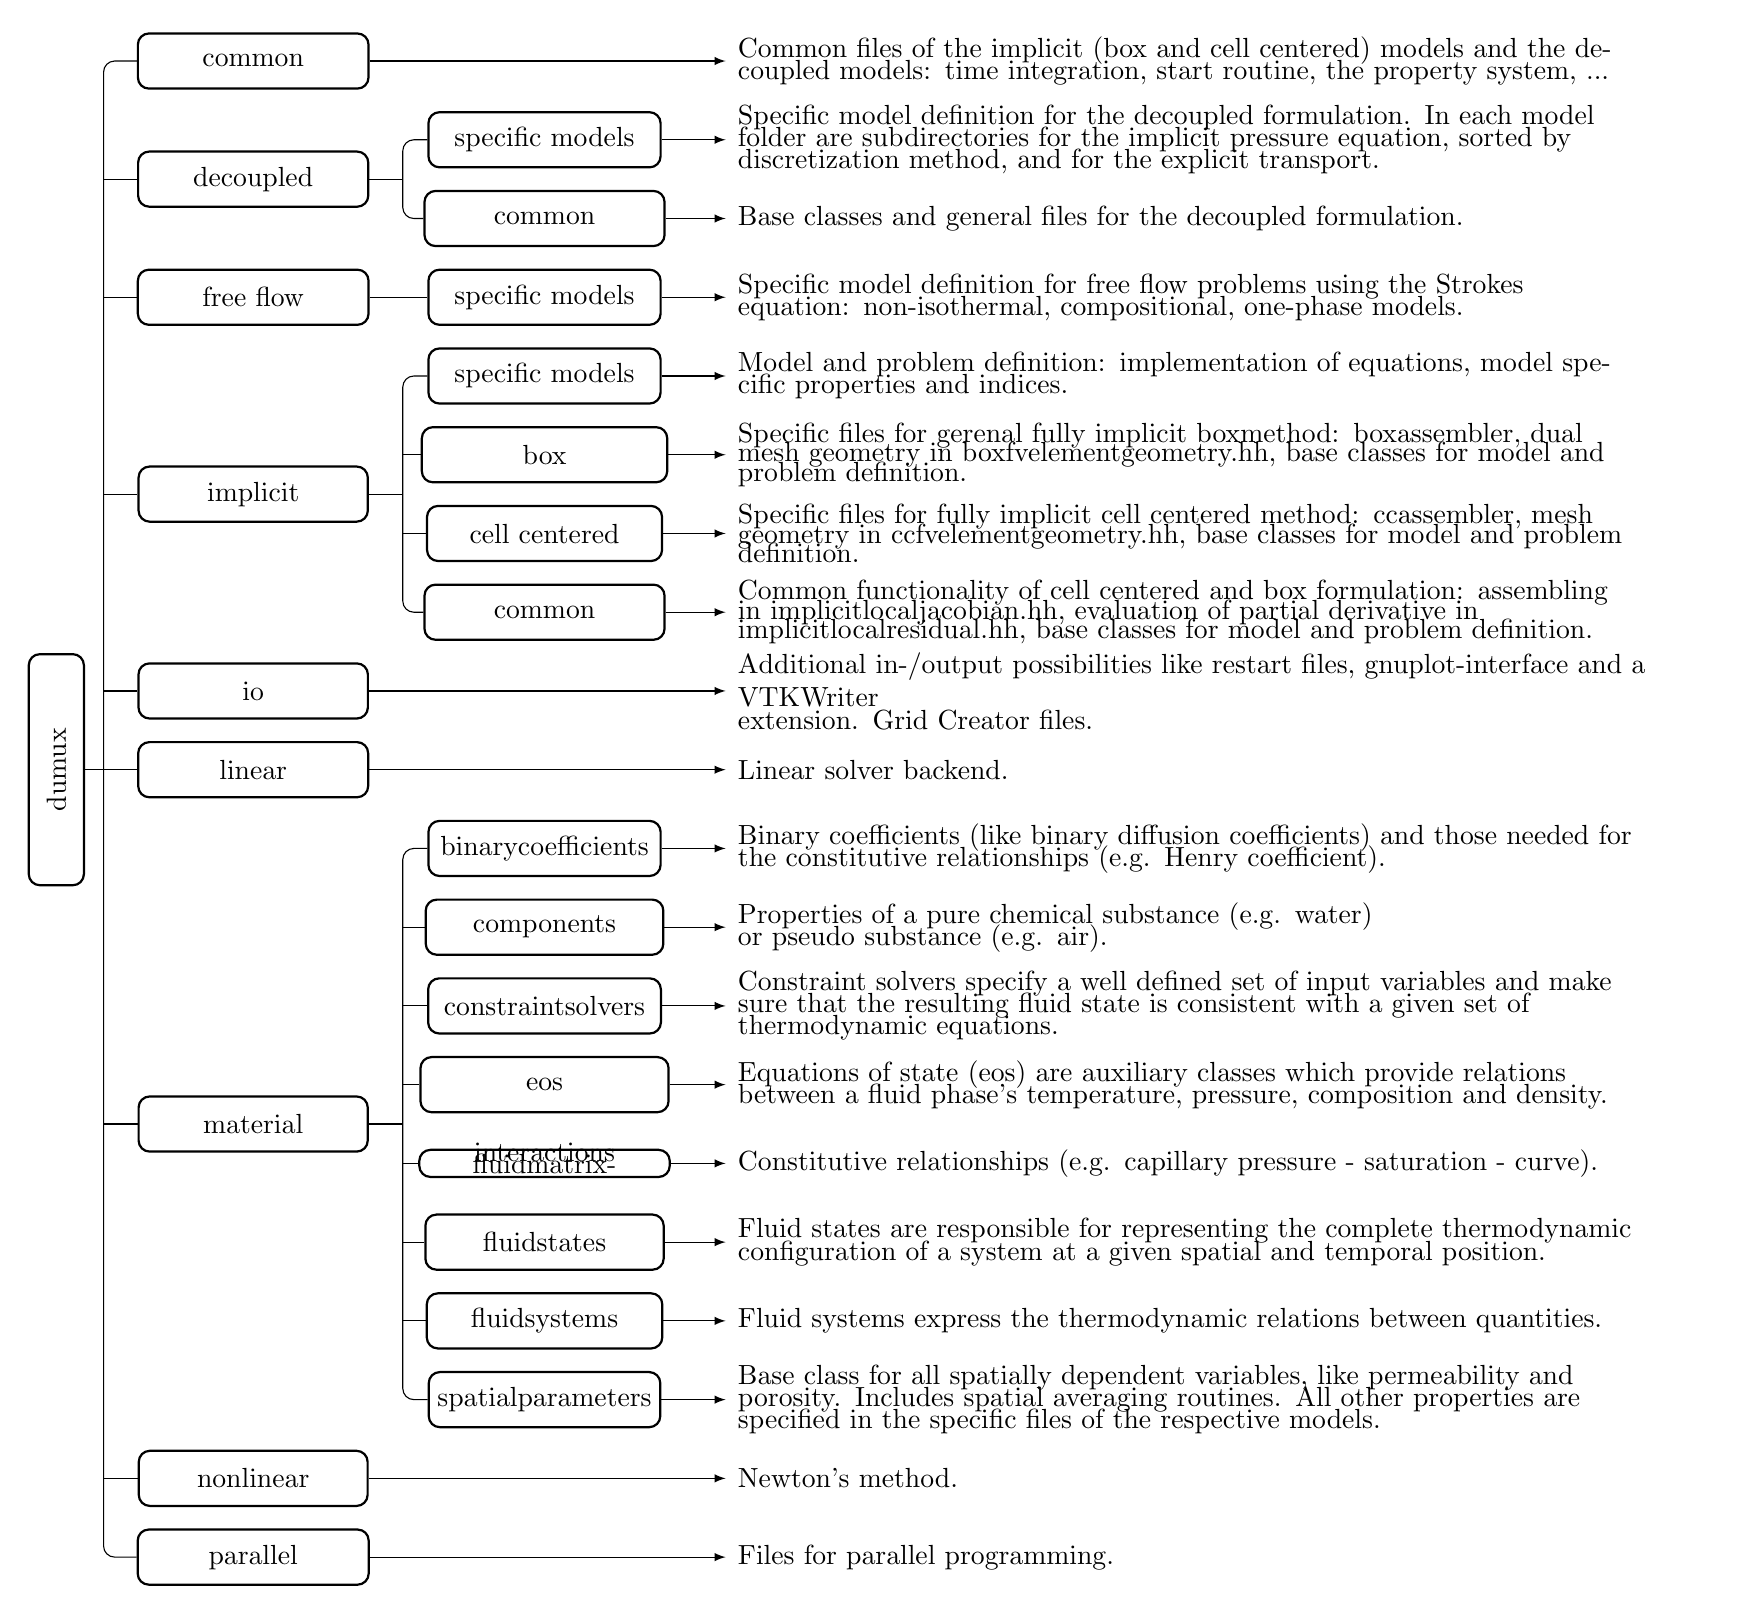
\begin{tikzpicture}[>=latex,inner xsep=0.15cm,rounded corners]
\node [minimum height=0.7cm,draw,inner xsep=0.94cm,rotate=90,thick] (d) at(-2,0) {dumux};
\node [minimum height=0.7cm,draw,inner xsep=1.03cm,thick] (lin) at(0.5,0) {linear};
\node [minimum height=0.7cm,draw,inner xsep=1.32cm,thick] (io) at(0.5,1) {io};

\node [minimum height=0.7cm,draw,inner xsep=0.87cm,thick] (imp) at(0.5,3.5) {implicit};
 \node [minimum height=0.7cm,draw,inner xsep=0.88cm,thick] (c1) at(4.2,2) {common};
 \node [minimum height=0.7cm,draw,inner xsep=0.54cm,thick] (cell) at(4.2,3) {cell centered};
 \node [minimum height=0.7cm,draw,inner xsep=1.28cm,thick] (box) at(4.2,4) {box};
 \node [minimum height=0.7cm,draw,inner xsep=0.33cm,thick] (spec1) at(4.2,5) {specific models};

\node [minimum height=0.7cm,draw,inner xsep=0.82cm,thick] (free) at(0.5,6) {free flow};
  \node [minimum height=0.7cm,draw,inner xsep=0.33cm,thick] (spec2) at(4.2,6) {specific models};

\node [minimum height=0.7cm,draw,inner xsep=0.7cm,thick] (dec) at(0.5,7.5) {decoupled};
 \node [minimum height=0.7cm,draw,inner xsep=0.88cm,thick] (c2) at(4.2,7) {common};
 \node [minimum height=0.7cm,draw,inner xsep=0.33cm,thick] (spec3) at(4.2,8) {specific models};

\node [minimum height=0.7cm,draw,inner xsep=0.82cm,thick] (c3) at(0.5,9) {common};

\node [minimum height=0.7cm,draw,inner xsep=0.82cm,thick] (m) at(0.5,-4.5) {material};
 \node [minimum height=0.7cm,draw,thick] (bin) at(4.2,-1) {binarycoefficients};
 \node [minimum height=0.7cm,draw,inner xsep=0.6cm,thick] (comp) at(4.2,-2) {components};
 \node [minimum height=0.7cm,draw,inner xsep=0.2cm,thick] (con) at(4.2,-3) {constraintsolvers};
 \node [minimum height=0.7cm,draw,inner xsep=1.34cm,thick] (eos) at(4.2,-4) {eos};
 \node [inner ysep=0.05cm,draw,text width=2cm,align=center,inner xsep=0.59cm,thick] (fi) at(4.2,-5) {fluidmatrix-\\[-16pt]interactions};
 \node [minimum height=0.7cm,draw,inner xsep=0.73cm,thick] (fstate) at(4.2,-6) {fluidstates};
 \node [minimum height=0.7cm,draw,inner xsep=0.56cm,thick] (fsys) at(4.2,-7) {fluidsystems};
 \node [minimum height=0.7cm,draw,inner xsep=0.11cm,thick] (s) at(4.2,-8) {spatialparameters};

\node [minimum height=0.7cm,draw,inner xsep=0.74cm,thick] (non) at(0.5,-9) {nonlinear};
\node [minimum height=0.7cm,draw,inner xsep=0.9cm,thick] (para) at(0.5,-10) {parallel};

\draw (d)--(lin);
\draw (-1.4,0)--(-1.4,9)--(c3);
\draw (-1.4,0)--(-1.4,-10)--(para);
\draw (-1.4,7.5)--(dec);
\draw (-1.4,6)--(free);
\draw (-1.4,3.5)--(imp);
\draw (-1.4,1)--(io);
\draw (-1.4,-4.5)--(m);
\draw (-1.4,-9)--(non);

\draw (dec)--(2.4,7.5);
\draw (spec3)--(2.4,8)--(2.4,7)--(c2);
\draw (free)--(spec2);
\draw (imp)--(2.4,3.5);
\draw (spec1)--(2.4,5)--(2.4,2)--(c1);
\draw (box)--(2.4,4);
\draw (cell)--(2.4,3);
\draw (m)--(2.4,-4.5);
\draw (bin)--(2.4,-1)--(2.4,-8)--(s);
\draw (comp)--(2.4,-2);
\draw (con)--(2.4,-3);
\draw (eos)--(2.4,-4);
\draw (fi)--(2.4,-5);
\draw (fstate)--(2.4,-6);
\draw (fsys)--(2.4,-7);

\draw [->](c3)--(6.5,9) node [right,text width=12.5cm,align=left]
  {Common files of the implicit (box and cell centered) models and the de-\\[-4pt]
   coupled models: time integration, start routine, the  property system, ...};
\draw [->](spec3)--(6.5,8) node [right,text width=12.5cm,align=left]
  {Specific model definition for the decoupled formulation. In each model \\[-4pt]
   folder are subdirectories for the implicit pressure  equation, sorted by \\[-4pt]discretization method, and for the explicit transport.};
\draw [->](c2)--(6.5,7) node [right,text width=12.5cm,align=left]
  {Base classes and general files for the decoupled formulation.};
\draw [->](spec2)--(6.5,6) node [right,text width=12.5cm,align=left]
  {Specific model definition for free flow problems using the Strokes \\[-4pt]
   equation: non-isothermal, compositional, one-phase models.};
\draw [->](spec1)--(6.5,5) node [right,text width=12.5cm,align=left]
  {Model and problem definition: implementation of equations, model spe-\\[-4pt]
   cific properties and indices.};
\draw [->](box)--(6.5,4) node [right,text width=12.5cm,align=left]
  {Specific files for gerenal fully implicit boxmethod: boxassembler, dual \\[-5pt]
   mesh geometry in boxfvelementgeometry.hh, base classes for model and \\[-5pt]problem definition.};
\draw [->](cell)--(6.5,3) node [right,text width=12.5cm,align=left]
  {Specific files for fully implicit cell centered method: ccassembler, mesh \\[-5pt]
   geometry in ccfvelementgeometry.hh, base classes for model and problem \\[-5pt]definition.};
\draw [->](c1)--(6.5,2) node [right,text width=12.5cm,align=left]
  {Common functionality of cell centered and box formulation: assembling \\[-5pt]
   in implicitlocaljacobian.hh, evaluation of partial derivative in \\[-5pt]implicitlocalresidual.hh, base classes for model and problem definition.};
\draw [->](io)--(6.5,1) node [right,text width=12.5cm,align=left]
  {Additional in-/output possibilities like restart files, gnuplot-interface and a VTKWriter \\[-4pt]
   extension. Grid Creator files.};
\draw [->](lin)--(6.5,0) node [right,text width=12.5cm,align=left] {Linear solver backend.};
\draw [->](bin)--(6.5,-1) node [right,text width=12.5cm,align=left]
  {Binary coefficients (like binary diffusion coefficients) and those needed for \\[-4pt]
   the constitutive relationships (e.g. Henry coefficient).};
\draw [->](comp)--(6.5,-2) node [right,text width=12.5cm,align=left]
  {Properties of a pure chemical substance (e.g. water) \\[-4pt]or pseudo substance (e.g. air).};
\draw [->](con)--(6.5,-3) node [right,text width=12.5cm,align=left]
  {Constraint solvers specify a well defined set of input variables and make \\[-4pt]
   sure that the resulting fluid state is consistent with a given set of \\[-4pt]thermodynamic equations.};
\draw [->](eos)--(6.5,-4) node [right,text width=12.5cm,align=left]
  {Equations of state (eos) are auxiliary classes which provide relations \\[-4pt]
   between a fluid phase's temperature, pressure, composition and density.};
\draw [->](fi)--(6.5,-5) node [right,text width=12.5cm,align=left]
  {Constitutive relationships (e.g. capillary pressure - saturation - curve).};
\draw [->](fstate)--(6.5,-6) node [right,text width=12.5cm,align=left]
  {Fluid states are responsible for representing the complete thermodynamic \\[-4pt]
   configuration of a system at a given spatial and temporal position.};
\draw [->](fsys)--(6.5,-7) node [right,text width=12.5cm,align=left]
  {Fluid systems express the thermodynamic relations between quantities.};
\draw [->](s)--(6.5,-8) node [right,text width=12.5cm,align=left]
  {Base class for all spatially dependent variables, like permeability and \\[-4pt]
   porosity. Includes spatial averaging routines. All other properties are \\[-4pt]
   specified in the specific files of the respective models.};
\draw [->](non)--(6.5,-9) node [right,text width=12.5cm,align=left]
  {Newton's method.};
\draw [->](para)--(6.5,-10) node [right,text width=12.5cm,align=left]
  {Files for parallel programming.};
\end{tikzpicture}
\caption{Structure of the directory \texttt{dumux} containing the \Dumux source files.
\todo[inline]{bei dieser Skizze sollten wir auch schauen ob die noch aktuell ist.}}
\label{fig:dumux-structure}
\end{sidewaysfigure}

\section{Setup of a New Folder and New Tests}

\paragraph{Setting up a New Folder}
In this section it is described how to set up a new folder and how to tell
the build system, that there is a new one.

\begin{enumerate}[1)]
 \item create new folder with content
 \item adapt the \verb+CMakeList.txt+ in the folder above and add a line with
       \verb+add_subdirectory(NEW\_FOLDER)+
 \item adapt the \verb+CMakeList.txt+ in the newly created folder and add your test
       (see below for more information)
 \item go to your \texttt{build}-directory and type \verb+make+ to
       reconfigure the system
\end{enumerate}

\paragraph{Adding a New Test Program}
\noindent To simply add a new executable use the following macro. The test will \emph{not} be built
automatically when running \texttt{ctest}. You have to compile it manually by
\texttt{make test\_program}.
\begin{verbatim}
add_executable_all(test\_program test\_program.cc)
\end{verbatim}

\noindent To add a test, which should be compiled when running \texttt{ctest}, use the
\texttt{add\_dumux\_test} macro. You can decide whether, the program should be run
after compiling or not.
Please note that the name of the test (first argument) must be unique, whereas the name
of the executable (second argument) can occur multiple times.
\begin{verbatim}
add_dumux_test(test\_program test\_program test\_program.cc
  test\_program # add this line, if the program should also be run
  )
\end{verbatim}

\noindent To add a test which should be run and compared to a reference solution when using
\texttt{ctest}, please use the following structure. The macro \texttt{\${CMAKE\_SOURCE\_DIR}}
gives the location of your source code. The macro \texttt{\${CMAKE\_CURRENT\_BINARY\_DIR}}
gives the current folder with the executable.
\begin{verbatim}
add_dumux_test(test\_program test\_program test\_program.cc
  ${CMAKE_SOURCE_DIR}/bin/runTest.sh
  ${CMAKE_SOURCE_DIR}/bin/fuzzycomparevtu.py
  LOCATION_TO_THE_REFERNCE_SOLUTION/test\_program-reference.vtu
  ${CMAKE_CURRENT_BINARY_DIR}/test\_program-00009.vtu
  ${CMAKE_CURRENT_BINARY_DIR}/test\_program)
\end{verbatim}

\paragraph{Committing a New older to SVN}
For those who work with Subversion (\texttt{svn}) and want to commit a newly setup folder to the repository some basics are
given in this paragraph. For further reading please check out the Subversion User Manual found at \cite{APACHE-SUBVERSION-HP}
where you will also find a "High Speed Turorial" in the appendix. \\
The four most important commands are \texttt{svn checkout}, \texttt{svn update},  \texttt{svn add}
and \texttt{svn commit}. The first one (\texttt{svn checkout}) you probably already know from the \Dumux installation.
It will create a copy of the trunk version from the svn server on your local system. Use \texttt{svn update} to get the
latest changes in the repository (commits from other users). In order to add a new folder to the repository the following
steps have to be taken:

\begin{enumerate}[1)]
\item \texttt{svn update}: The first step is to update your \Dumux. You should execute this command in your
      dumux-stable or dumux-devel folder.
\item \texttt{svn add --depth=empty YOURFOLDER}: This command adds the folder without its content.
\item In your folder: use \texttt{svn add YOURFILES} to add your files. Generally, you should only add
      your header files (.hh), your source files (.cc), your input file (.input), if required your
      grid file (.dgf) or if necessary other text-based files. Please do not upload (large) binary files.
\item Type \texttt{svn status} in your \texttt{dumux}-root directory the see all the file changes.
      \texttt{?} indicates possible forgotten files. Make sure that you include all necessary
      files in your commit.
\item Use \texttt{svn commit} from the directory level containing your folder. This uploads all your changes to the
      svn server. You will be asked to briefly explain the content of your commit in an editor.
\end{enumerate}

\section{Parameters in \Dumux}
\label{sc_parameterfiles}
Simulation parameters can be parsed to the program via a parameter file or the command line.
A list of all available parameters is provided in the Doxygen documentation
of the file \texttt{parameterfile}, which is accessible via \texttt{Modules -> Parameters}.

After having run the example application from section \ref{quick-start-guide} you will
get the following output at the end of the simulation run
\footnote{If you did not get the output, restart the application the following way:
\texttt{./test{\_}box2p -PrintParameters true},
this will print the parameters once your simulation is finished}:
\begin{lstlisting}[style=Bash]
# Run-time specified parameters:
[ Grid ]
File = "./grids/test_2p.dgf"
[ Implicit ]
EnableJacobianRecycling = "1"
EnablePartialReassemble = "1"
[ Problem ]
Name = "lensbox"
[ SpatialParams ]
LensLowerLeftX = "1.0"
LensLowerLeftY = "2.0"
LensUpperRightX = "4.0"
LensUpperRightY = "3.0"
[ TimeManager ]
DtInitial = "250"
TEnd = "3000"
# DEPRECATED run-time specified parameters:
PrintParameters = "1"
# Replace by:
[ TimeManager ]
PrintParameters = "1"
# Compile-time specified parameters:
[ Implicit ]
EnableHints = "0"
MassUpwindWeight = "1"
MaxTimeStepDivisions = "10"
MobilityUpwindWeight = "1"
NumericDifferenceMethod = "1"
UseTwoPointFlux = "0"
[ LinearSolver ]
MaxIterations = "250"
PreconditionerRelaxation = "1"
ResidualReduction = "1e-06"
Verbosity = "0"
[ Newton ]
WriteConvergence = "0"
[ Problem ]
EnableGravity = "1"
[ TimeManager ]
MaxTimeStepSize = "1.79769e+308"
[ Vtk ]
AddVelocity = "0"
# UNUSED parameters:
ImportantVariable = "1"
\end{lstlisting}

A number of things can be learned:
\begin{itemize}
  \item \emph{run-time} parameters can be changed without re-compiling
  \item \emph{deprecated run-time} parameters will be removed in the next release
  \item \emph{compile-time} parameters cannot be overwritten by the input file
  \item \emph{unused} are not used by the simulation (maybe typo or wrong group)
\end{itemize}

All applications have a help message which you can read by giving
\texttt{--help} as a command line argument to the application.

For further details, please have a look for \texttt{Dune::ParameterTree}
in the \Dune documentation.

\section{Restart \Dumux Simulations}
\label{sc_restartsimulations}

\Dumux has some experimental support for check-pointing (restarting paused/stopped/crashed simulations).
You can restart a \Dumux simulation from any time point where a VTK file was written out.
This is currently only supported for sequential, non-adaptive simulations. For adaptive simulation
the full hierarchical grid has to be stored. This is usually done with the grid's \texttt{BackupRestoreFacility}.
There is currently no special support by \Dumux for that, but it is possible to implement
a restart using \texttt{BackupRestoreFacility} with plain Dune.

For VTK files the output can be read with the free function \texttt{loadSolution}. Grids can be read with
the \texttt{Dumux::VTKReader} or you can simply recreate the grid as you did in the first simulation run.

Unfortunately, writing double-precision floating point numbers to VTK files is only available with Dune master (will be in 2.7).
That's why we currently only support single precision restart, meaning some information will be lost if you are computing
in double precision.

The restart capabilities will hopefully be improved in future versions of \Dumux 3.
We are happy about any contributions (especially HDF5 / XDMF support, improvement of VTK support).

\section{Developing \Dumux}
\label{sc_developingdumux}

\subsection{Communicate with \Dumux Developers}

\paragraph{Issues and Bug Tracking}
The bug-tracking system \emph{GitLab Issues} offers the possibility to report bugs or discuss new development requests.
Feel free to register (if you don't have a \emph{Git} account already) and to constribute
at \url{https://git.iws.uni-stuttgart.de/dumux-repositories/dumux/issues}.

\paragraph{Commits, Merges, etc.}
To be up-to-date with the latest changes made to any git-repository you can use RSS Feeds.
Simply click on \emph{Issues} or \emph{Activity} and then select a tab you are interested in
and use your favorite RSS-application for receiving the news.

\paragraph{Automatic Testing Dashboard}
The automatic testing using \emph{BuildBot} helps to constantly check the
\Dumux problems for compiling and running correctly. It is available at
\url{https://git.iws.uni-stuttgart.de/buildbot/#/builders}.

\paragraph{The General Mailing List:}
If you have questions, specific problems (which you really struggle to solve on your own),
or hints for the \Dumux-developers, please contact the mailing list \url{dumux@iws.uni-stuttgart.de}.
You can subscribe to the mailing list via
\url{https://listserv.uni-stuttgart.de/mailman/listinfo/dumux}, then you
will be informed about upcoming releases or events.

\subsection{Coding Guidelines}
Writing code in a readable manner is very important, especially
for future code developers (e.g. for adding features, debugging, etc.).
For the style guide and instructions how to contribute to \Dumux visit
\url{https://git.iws.uni-stuttgart.de/dumux-repositories/dumux/blob/master/CONTRIBUTING.md}.


\subsection{Tips and Tricks}
\Dumux users and developers at the LH2 are also referred to the internal Wiki for
more information.

\paragraph{Optimized computation vs debugging}
\Dune and \Dumux are built with the help of \texttt{dunecontrol}, as explained on page \pageref{buildIt}.
Per default, \Dumux is compiled using optimization options, which leads to faster runtimes but is unsuitable
for debugging. For debug opts you can set \texttt{DCMAKE_BUILD_TYPE} to \texttt{Debug} or \texttt{RelWithDebInfo}
in your options file. You can also do this in any of the \texttt{CMakeLists.txt} in Dumux by adding:

\begin{lstlisting}[style=Shell]
set(CMAKE_BUILD_TYPE Debug)
\end{lstlisting}

Afterwards rerun cmake again (run cmake <path-to-build-dir>).

\paragraph{Dunecontrol for selected modules}
A complete build using \texttt{dunecontrol} takes some time. In many cases not all modules need to be re-built.
Pass the flag \texttt{--only=dumux} to \texttt{dunecontrol} for configuring or building only \Dumux. A more
complex example would be the use of an additional module. Then you have to configure and build only \Dune{}-grid
and \Dumux by adding \texttt{--only=MODULE,dumux}.

\paragraph{Patching Files or Modules}
If you want to send changes to an other developer of \Dumux providing patches
can be quite smart. To create a patch simply type:
\begin{lstlisting}[style=Bash]
$ git diff > PATCHFILE
\end{lstlisting}
\noindent which creates a text file containing all your changes to the files
in the current folder or its subdirectories.
To apply a patch in the same directory type:
\begin{lstlisting}[style=Bash]
$ patch -p1 < PATCHFILE
\end{lstlisting}

%TODO: currently, no DUNE patches necessary! Thus, this section is commented and the missing refrence would be bad.
% Uncomment the following statement again when patches might be necessary.
% See \ref{sc:patchingDUNE} if you need to apply patches to \Dumux or \Dune.

\paragraph{File Name and Line Number by Predefined Macro}
If you want to  know where some output or debug information came from, use the predefined
macros \texttt{\_\_FILE\_\_} and \texttt{\_\_LINE\_\_}:
\begin{lstlisting}[style=DumuxCode]
std::cout << "# This was written from "<< __FILE__ << ", line " << __LINE__ << std::endl;
\end{lstlisting}

\paragraph{Using \Dune Debug Streams}
\Dune provides a helpful feature, for keeping your debug-output organized.
It uses simple streams like \texttt{std::cout}, but they can be switched on and off
for the whole project. You can chose five different levels of severity:
\begin{verbatim}
5 - grave (dgrave)
4 - warning (dwarn)
3 - info (dinfo)
2 - verbose (dverb)
1 - very verbose (dvverb)
\end{verbatim}
\noindent They are used as follows:
\begin{lstlisting}[style=DumuxCode]
// define the minimal debug level somewhere in your code
#define DUNE_MINIMAL_DEBUG_LEVEL 4
Dune::dgrave << "message"; // will be printed
Dune::dwarn << "message"; // will be printed
Dune::dinfo << "message"; // will NOT be printed
\end{lstlisting}

\paragraph{Make headercheck:}
To check one header file for all necessary includes to compile the contained code, use \texttt{make headercheck}.
Include the option \texttt{-DENABLE\_HEADERCHECK=1} in your opts file and run \texttt{dunecontrol}.
Then go to the top level in your build-directory and type \texttt{make headercheck} to check all headers
or press 'tab' to use the auto-completion to search for a specific header.

\section{External Tools}
\label{sc_externaltools}

\subsection{Eclipse}
There is an Eclipse style file which can be used for \Dumux.
\begin{enumerate}
  \item open in eclipse: \texttt{Window} $\rightarrow$ \texttt{Preferences} $\rightarrow$
        \texttt{C/C++}  $\rightarrow$ \texttt{Code Style} $\rightarrow$ \texttt{Formatter}
  \item press the \texttt{Import} button
  \item choose the file \texttt{eclipse\_profile.xml} from your dumux-devel directory
  \item make sure that now \Dumux is chosen in \texttt{Select a profile}
\end{enumerate}


\subsection{Git}
Git is a version control tool which we use.
The basic Git commands are:
\begin{itemize}
  \item \texttt{git checkout} receive a specified branch from the repository
  \item \texttt{git clone} clone a repository; creates a local copy
  \item \texttt{git diff} to see the actual changes compared to your last commit
  \item \texttt{git pull} pull changes from the repository; synchronizes the
  repository with your local copy
  \item \texttt{git push} push comitted changes to the repository;  synchronizes
  your local copy with the repository
  \item \texttt{git status} to check which files/folders have been changed
  \item \texttt{git gui} graphical user interface, helps selecting changes for
  a commit
\end{itemize}


\subsection{Gnuplot}
\label{gnuplot}
A gnuplot interface is available to plot or visualize results during a simulation run.
This is achieved with the help of the class provided in \texttt{io/gnuplotinterface.hh}.

To use the gnuplot interface you have to make some modifications in your file, e.g., your main file.

First, you have to include the corresponding header file for the gnuplot interface. 
\begin{lstlisting}[style=DumuxCode]
#include <dumux/io/gnuplotinterface.hh
\end{lstlisting}

Second, you have to define an instance of the class GnuplotInterface (e.g. called \texttt{gnuplot}).
\begin{lstlisting}[style=DumuxCode]
Dumux::GnuplotInterface<double> gnuplot;
\end{lstlisting}

Extract the variables you want to plot (in the example below \texttt{x} and \texttt{y}), e.g., after the time loop. 
The actual plotting is done using the method of the gnuplot interface.

Example:
\begin{lstlisting}[style=DumuxCode]
gnuplot.resetPlot();                             // reset the plot
gnuplot.setXRange(0.0, 72000.0);                 // specify xmin and xmax  
gnuplot.setYRange(0.0, 1.0);                     // specify ymin and ymax
gnuplot.setXlabel("time [s]");                   // set xlabel
gnuplot.setYlabel("mole fraction mol/mol");  // set ylabel

// set x-values, y-values, the name of the data file and the Gnupot options
gnuplot.addDataSetToPlot(x, y, "N2_left.dat", options); 

gnuplot.plot("mole_fraction_N2");                // set the name of the output file
\end{lstlisting}

It is also possible to add several data sets to one plot by calling \texttt{addDataSetToPlot()} more than once.
For more information have a look into a test including the gnuplot interface header file or
the header file itself (\texttt{dumux/io/gnuplotinterface.hh}).


\subsection{Gstat}
Gstat is an open source software tool which generates geostatistical random fields (see \url{www.gstat.org}).
In order to use gstat, execute the \texttt{bin/installexternal.sh} from your \Dumux root
directory or donwload, unpack and install the tarball from the gstat-website.
Then rerun cmake (in the second case set \texttt{GSTAT\_ROOT} in your input file to the
path where gstat is installed).


\subsection{ParaView}
\paragraph{Reload Button:}
There are scripts to reload \texttt{*.pvd} or series of {\texttt{*.vtu} files since ParaView 4.2.
The scripts can be found
\href{http://markmail.org/message/exxynsgishbvtngg#query:+page:1+mid:rxlwxs7uqrfgibyv+state:results}{\texttt{under this link}}.
Just save the specific code portion in a file and load it via \texttt{Macros} $\rightarrow$ \texttt{Add new macro}.

\paragraph{Guide:}
Since ParaView 4.3.1 The ParaView Guide is partly
available for free download, see \url{http://www.paraview.org/documentation/}.
It corresponds to the ParaView book, only without three application chapters.
Attention, its size is 180 MiB.

\section{Assembling the linear system}
\label{sc_linearsystem}
The physical system is implemented as the mathematical differential equation in
local operators. \Dumux generates the linear system automatically. Read on, to
learn what is done internally.

\subsection{Newton's method}
The differential equations are implemented in the residual form. All terms are
on the left hand side and are summed up. The terms contain values for the primary
variables which are part of the solution vector $\textbf{u}$. The sum of the terms
is called residual $\textbf{r}(\textbf{u})$ which is a function of the solution. For
example:
\begin{align*}
\underbrace{
  \phi \frac{\partial \varrho_\alpha S_\alpha}{\partial t}
 -
 \text{div} \left(
 \varrho_\alpha \frac{k_{r\alpha}}{\mu_\alpha} \mbox{\bf K}
 \left(\grad\, p_\alpha - \varrho_{\alpha} \mbox{\bf g} \right)
 \right) - q_\alpha} _
{=: \, \textbf{r}(\textbf{u})}
= 0
\end{align*}

We don't know the solution $\textbf{u}$, so we use the iterative Newton's method to
obtain a good estimate of $\textbf{u}$. We start with an initial guess $\textbf{u}^0$ and
calculate it's residual $\textbf{r}(\textbf{u}^0)$. To minimize the error, we calculate
the derivative of the residual with respect to the solution. This is the Jacobian
matrix
\begin{align*}
  \frac{\text{d}}{\text{d}\textbf{u}}\textbf{r} \left(\textbf{u}^i\right)
  = J_{\textbf{r} \left(\textbf{u}^i\right)}
  = \left(\frac{\text{d}}{\text{d}\textbf{u}^i_m}\textbf{r} \left(\textbf{u}^i\right)_n\right)_{m,n}
\end{align*}
with $i$ denoting the Newton iteration step.
Each column is the residual derived with respect to the $m$th entry of $\textbf{u}^i$.

The Jacobian indicates the direction where the residual increases. By solving the
linear system
\begin{align*}
  J_{\textbf{r}(\textbf{u}^i)} \cdot \textbf{x}^i = \textbf{u}^i
\end{align*}
we calculate the direction of maximum growth $\textbf{x}^i$. We subtract it from
our current solution to get a new, better solution
$\textbf{u}^{i+1} = \textbf{u}^i - \textbf{x}^i$.

We repeat the calculation of of the Jacobian $J_{\textbf{r}(\textbf{u}^i)}$ and the
direction of maximum growth $\textbf{x}^i$ until our approximated solution becomes good enough.

\subsection{Structure of matrix and vectors}
To understand the meaning of an entry in the matrix or the vector of the linear system, we have
to define their structure. Both have a blocking structure. Each block contains the degrees of
freedom (also called variable or unknown) for a sub-control volume. The equation index is used
to order of the degrees of freedom. For each sub-control volume we have one block. The mapper is
used to order the blocks.

\begin{figure}[htbp]
\begin{center}
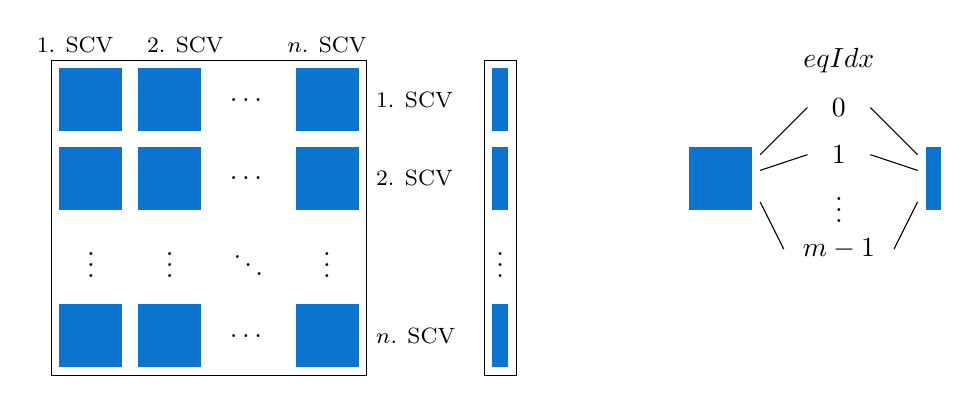
\begin{tikzpicture}[fill=dumuxBlue]
  %% blocking structure
  % matrix
  \node at (0.3,4.2){\footnotesize 1. SCV};
  \node at (1.7,4.2){\footnotesize 2. SCV};
  \node at (3.5,4.2){\footnotesize $n$. SCV};

  \draw (0,0) rectangle (4,4);
  
  \fill (0.1,3.1) rectangle (0.9,3.9);
  \fill (1.1,3.1) rectangle (1.9,3.9);
  \node at (2.5,3.5) {$\dots$};
  \fill (3.1,3.1) rectangle (3.9,3.9);
  \node at (4,3.5) [right]{\footnotesize 1. SCV};

  \fill (0.1,2.1) rectangle (0.9,2.9);
  \fill (1.1,2.1) rectangle (1.9,2.9);
  \node at (2.5,2.5) {$\dots$};
  \fill (3.1,2.1) rectangle (3.9,2.9);
  \node at (4,2.5) [right]{\footnotesize 2. SCV};

  \node at (0.5,1.5) {$\vdots$};
  \node at (1.5,1.5) {$\vdots$};
  \node at (2.5,1.5) {$\ddots$};
  \node at (3.5,1.5) {$\vdots$};

  \fill (0.1,0.1) rectangle (0.9,0.9);
  \fill (1.1,0.1) rectangle (1.9,0.9);
  \node at (2.5,0.5) {$\dots$};
  \fill (3.1,0.1) rectangle (3.9,0.9);
  \node at (4,0.5) [right]{\footnotesize $n$. SCV};

  % vector
  \draw (5.5,0) rectangle (5.9,4);
  \fill (5.6,3.1) rectangle (5.8,3.9);
  \fill (5.6,2.1) rectangle (5.8,2.9);
  \node at (5.7,1.5) {$\vdots$};
  \fill (5.6,0.1) rectangle (5.8,0.9);
  
  %% intra-block structure
  \fill (8.1,2.1) rectangle (8.9,2.9);
  \draw (9,2.8) -- (9.6,3.4);
  \draw (9,2.6) -- (9.6,2.8);
  \draw (9,2.2) -- (9.3,1.6);
  
  \node at (10,4) {${eqIdx}$};
  \node at (10,3.4) {$0$};
  \node at (10,2.8) {$1$};
  \node at (10,2.2) {$\vdots$};
  \node at (10,1.6) {$m-1$};
  
  \fill (11.1,2.1) rectangle (11.3,2.9);
  \draw (11,2.8) -- (10.4,3.4);
  \draw (11,2.6) -- (10.4,2.8);
  \draw (11,2.2) -- (10.7,1.6);
\end{tikzpicture}
\end{center}
\caption{Structure of matrix and vector, left blocking structure, right within block}
\end{figure}

Accessing entries follows this structure. You can access the pressure value in the third sub-control volume in
a vector \lstinline{sol} with \lstinline{sol[2][pressureIdx]}.


\chapter{Advanced \Dumux\ -- Detailed Instructions}
This chapter contains detailed information for those who are interested
in deeper modifications of underlying \Dumux models, classes, functions, etc.
\section[The \Dumux Models]{Physical and Numerical Models Available in \Dumux}
\todo[inline]{Evtl. könnten wir das in zwei kapitel aufsplitten? Physical und numerical
 models}

\subsection{Physical and Mathematical Description}

Characteristic of compositional multiphase models is that the phases
are not only matter of a single chemical substance. Instead, their
composition in general includes several species, and for the mass transfer,
the component behavior is quite different from the phase behavior. In the following, we
give some basic definitions and assumptions that are required for the
formulation of the model concept below. As an example, we take a
three-phase three-component system water-NAPL-gas
\cite{A3:class:2002a}. The modification for other multicomponent
systems is straightforward and can be found, e.\ g., in
\cite{A3:bielinski:2006,A3:acosta:2006}.

\subsubsection{Basic Definitions and Assumptions for the Compositional
  Model Concept}
\textbf{Components:}
The term {\it component} stands for constituents of the phases which
can be associated with a unique chemical species, or, more generally, with
a group of species exploiting similar physical behavior. In this work, we
assume a water-gas-NAPL system composed of the phases water (subscript
$\text{w}$), gas ($\text{g}$), and NAPL ($\text{n}$). These phases are
composed of the components water (superscript $\text{w}$), air
($\text{a}$), and the organic contaminant ($\text{c}$) (see Fig.\
\ref{fig:phaseMassEnergyTransfer}).

\begin{figure}
  \centering
  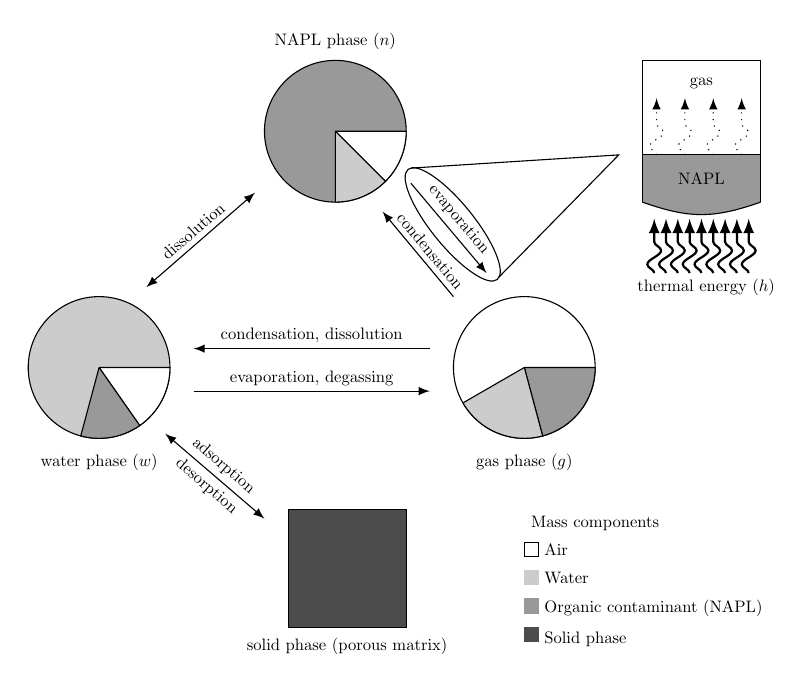
\begin{tikzpicture} [>=latex,scale=0.6, every node/.style={transform shape}]
    % Ellipse 1 solid
    \coordinate (A) at (1,-0.5);
    \draw [fill=black!70](A) rectangle(3.5,2) node at(2.25,-0.9) {solid phase (porous matrix)};
    % Ellipse 2 water
    \coordinate (B) at (-3,5);
    \draw [fill=black!20](B) circle(1.5cm);
    \node [yshift=5mm]at(-3,2.5){water phase $(w)$};
    \draw[fill=white] (B)--+(1.5,0)arc(0:-55:1.5cm)--(B);
    \draw[fill=black!40] (B)--+(-55:1.5cm)arc(-55:-105:1.5cm)--(B);
    % Ellipse 3 gas
    \coordinate (C) at (6,5);
    \draw [](C) circle (1.5cm);
    \node[yshift=5mm]at(6,2.5){gas phase $(g)$};
    \draw [fill=black!40](C)--+(1.5,0)arc(0:-75:1.5cm)--(C);
    \draw [fill=black!20] (C)--+(-75:1.5cm)arc(-75:-150:1.5cm)--(C);
    % Ellipse 4 napl
    \coordinate (D) at (2,10);
    \draw [fill=black!40](D) circle (1.5cm);
    \node[yshift=5mm]at(2,11.4){NAPL phase $(n)$};
    \draw [fill=white](D)--+(1.5,0)arc(0:-45:1.5cm)--(D);
    \draw [fill=black!20] (D)--+(0,-1.5)arc(-90:-45:1.5cm)--(D);
    % arrows
    %A-B
      \draw [<->,white](0.5,1.8)--(-1.6,3.6) node[black,above,sloped,pos=0.5]{adsorption};
      \draw [<->](0.5,1.8)--(-1.6,3.6) node[below,sloped,pos=0.5]{desorption};
    %B-C
      \draw[<-](-1,5.4)--(4,5.4)node[above,sloped,pos=0.5]{condensation, dissolution};
      \draw[->](-1,4.5)--(4,4.5)node[above,sloped,pos=0.5]{evaporation, degassing};
    %B-D
      \draw[<->](-2,6.7)--(0.3,8.7)node[above,sloped,pos=0.5]{dissolution};
    %D-C
      \draw[->](3.6,8.9)--(5.2,7)node[above,sloped,pos=0.5]{evaporation};
      \draw[rotate around={-51:(4,6.8)}](3.35,7.95) ellipse (1.5cm and 0.45cm);  %Ellipse um evaporation
      \draw (3.6,9.22)--(8,9.5)--(5.45,6.9);
      \draw[<-](3,8.3)--(4.5,6.5)node[above,sloped,pos=0.55]{condensation};
    % thermal energy
    \filldraw [black!40](8.5,9.5)rectangle(11,8.5);
    \draw (8.5,9.5)rectangle(11,11.5);
    \draw (8.5,9.5)--(8.5,8.5);
    \draw (11,9.5)--(11,8.5);
    \draw [decorate,decoration={bent,aspect=0.4,amplitude=6},fill=black!40](11,8.5)--(8.5,8.5);
    \foreach \x in {8.75,9,...,10.8}
    \draw [->,decorate,decoration={snake,post length=2mm},thick](\x,7)--(\x,8.15);
    \foreach \x in {8.8,9.4,10,10.6}
    \draw [->,dotted,decorate,decoration={snake,post length=2mm}](\x,9.5)--(\x,10.7);
    \node at(9.75,11){gas};
    \node at(9.75,9){NAPL};
    \node at(9.85,6.7){thermal energy $(h)$};
    % legende
    \node at (7.5,1.7){Mass components};
    \draw[](6,1)rectangle +(0.3,0.3) node at(6.3,1.15) [right]{Air};
    \filldraw[black!20](6,0.4) rectangle +(0.3,0.3) node at (6.3,0.55)[black,right]{Water};
    \filldraw[black!40](6,-0.2) rectangle +(0.3,0.3) node at (6.3,-0.1)[right,black]{Organic contaminant (NAPL)};
    \filldraw[black!70](6,-0.8) rectangle +(0.3,0.3) node at (6.3,-0.75)[right,black]{Solid phase};
  \end{tikzpicture}
  \caption{Mass and energy transfer between the phases}
  \label{fig:phaseMassEnergyTransfer}
\end{figure}

\textbf{Equilibrium:}
For the non-isothermal multiphase processes in porous media under
consideration, we state that the assumption of local thermal
equilibrium is valid since flow velocities are small. We neglect
chemical reactions and biological decomposition and assume chemical
equilibrium.  Mechanical equilibrium is not valid in a porous medium,
since discontinuities in pressure can occur across a fluid-fluid
interface due to capillary effects.

\textbf{Notation:} The index $\alpha \in \{\text{w}, \text{n}, \text{g}\}$ refers
to the phase, while the superscript $\kappa \in \{\text{w}, \text{a}, \text{c}\}$ refers
to the component. \\
\begin{tabular}{llll}
$p_\alpha$ & phase pressure & $\phi$ & porosity \\
$T$ & temperature & $K$ & absolute permeability tensor \\
$S_\alpha$ & phase saturation & $\tau$ & tortuosity \\
$x_\alpha^\kappa$ & mole fraction of component $\kappa$ in phase $\alpha$ & $\boldsymbol{g}$ & gravitational acceleration \\
$X_\alpha^\kappa$ & mass fraction of component $\kappa$ in phase $\alpha$ & $q^\kappa_\alpha$ & volume source term of $\kappa$ in $\alpha$ \\
$\varrho_{\text{mol},\alpha}$ & molar density of phase $\alpha$ & $u_\alpha$ & specific internal energy \\
$\varrho_{\alpha}$ & mass density of phase $\alpha$ & $h_\alpha$ & specific enthalpy \\
$M$ & molar mass of a phase or component & $c_\text{s}$ & specific heat enthalpy \\
$k_{\text{r}\alpha}$ & relative permeability & $\lambda_\text{pm}$ & heat conductivity \\
$\mu_\alpha$ & phase viscosity & $q^h$ & heat source term \\
$D_\alpha^\kappa$ & diffusivity of component $\kappa$ in phase $\alpha$ & $\boldsymbol{v}_{a,\alpha}$  & advective velocity \\
$\boldsymbol{v}_\alpha$ & velocity (Darcy or free flow)& & \\
\end{tabular}


\subsubsection{Balance Equations}
For the balance equations for multicomponent systems, it is in many
cases convenient to use a molar formulation of the continuity
equation. Considering the mass conservation for each component allows
us to drop source/sink terms for describing the mass transfer between
phases. Then, the
molar mass balance can be written as:
%
\begin{multline}
  \label{A3:eqmass1}
 \phi \frac{\partial (\sum_\alpha \varrho_{\text{mol}, \alpha}
    x_\alpha^\kappa S_\alpha )}{\partial t}
 - \sum\limits_\alpha \Div \left\lbrace \frac{k_{\text{r}
        \alpha}}{\mu_\alpha} \varrho_{\text{mol}, \alpha}
    x_\alpha^\kappa \textbf{K} (\grad p_\alpha -
    \varrho_{\alpha} \boldsymbol{g}) \right\rbrace  \\
  %
  %
 - \sum\limits_\alpha \Div \left\lbrace \tau \phi S_\alpha D_\alpha^\kappa \varrho_{\text{mol},
      \alpha} \grad x_\alpha^\kappa \right\rbrace
 - q^\kappa = 0, \qquad \kappa \in \{\text{w,a,c}\}.
\end{multline}

The component mass balance can also be written in terms of mass fractions
by replacing molar densities by mass densities and mole by mass fractions.
To obtain a single conserved quantity in the temporal derivative, the total
concentration, representing the mass of one component per unit volume, is defined as
\begin{displaymath}
C^\kappa = \sum_\alpha \phi S_\alpha \varrho_{\text{mass},\alpha} X_\alpha^\kappa \; .
\end{displaymath}
Using this definition, the component mass balance is written as:

\begin{multline}
  \label{A3:eqmass2}
    \frac{\partial C^\kappa}{\partial t} =
  \sum\limits_\alpha \Div \left\lbrace \frac{k_{\text{r}
        \alpha}}{\mu_\alpha} \varrho_{\text{mass}, \alpha}
    X_\alpha^\kappa \textbf{K} (\grad p_\alpha +
    \varrho_{\text{mass}, \alpha} \boldsymbol{g}) \right\rbrace  \\
  %
  %
   + \sum\limits_\alpha \Div \left\lbrace \tau \phi S_\alpha D_\alpha^\kappa \varrho_{\text{mass},
      \alpha} \frac{M^\kappa}{M_\alpha} \grad x_\alpha^\kappa \right\rbrace
 + q^\kappa = 0, \qquad \kappa \in \{\text{w,a,c}\}.
\end{multline}


In the case of non-isothermal systems, we further have to balance the
thermal energy. We assume fully reversible processes, such that entropy
is not needed as a model parameter. Furthermore, we neglect
dissipative effects and the heat transport due to molecular
diffusion. The energy balance can then be
formulated as:
%
\begin{multline}
  \label{A3:eqenergmak1}
  \phi \frac{\partial \left( \sum_\alpha \varrho_{\alpha}
      u_\alpha S_\alpha \right)}{\partial t} + \left( 1 -
    \phi \right) \frac{\partial \varrho_{\text{s}} c_{\text{s}}
    T}{\partial t}
 - \Div \left( \lambda_{\text{pm}} \grad T \right)
   \\
   - \sum\limits_\alpha \Div \left\lbrace \frac{k_{\text{r}
        \alpha}}{\mu_\alpha} \varrho_{\alpha} h_\alpha
    K \left( \grad p_\alpha - \varrho_{\alpha}
      \boldsymbol{g} \right) \right\rbrace
 - q^h \; = \; 0.
\end{multline}

In order to close the system, supplementary constraints for capillary pressure, saturations and mole
fractions are needed, \cite{A3:helmig:1997}.
According to the Gibbsian phase rule, the number of degrees of freedom
in a non-isothermal compositional multiphase system is equal to the
number of components plus one. This means we need as many independent
unknowns in the system description. The
available primary variables are, e.\ g., saturations, mole/mass
fractions, temperature, pressures, etc.

\subsection{Available Models}
The following description of the available models is automatically extracted
from the Doxygen documentation.

\todo[inline]{Die Modelle waren etwas uneinheitlich von der Notation (ich habe
  hier auch gerade das entsprechende ToDo entfernt). Das ist naturlich jetzt
  nicht mehr so schlimm, da die Modelle nicht mehr untereinander auftauchen,
  allerdings wird auch die Fehlersuche schwieriger (aus dem Auge aus dem Sinn).}

\todo[inline]{evtl. entferne Unterkapitel. Einfugen der Modelliste, die könnte
  in ahnlicher Form auch aufs doxygen? Update der Liste in die Release Manager
  Tasks ubernehmen}

\subsubsection{Fully-Implicit Models}

The fully-implicit models described in this section are using the box or the
cell centered finite volume method as described in section \ref{box} and \ref{cc}
for spatial and the implicit Euler
method as temporal discretization. The models themselves are located in
subdirectories of \texttt{dumux/implicit} of the \Dumux distribution.

\subsubsection{Decoupled Models}
%
The basic idea the so-called decoupled models have in common is to reformulate the
equations of multi-phase flow (e.g. Eq. \ref{A3:eqmass1}) into one equation for
pressure and equations for phase-/component-/etc. transport. The pressure equation
is the sum of the mass balance equations and thus considers the total flow of the
fluid system. The new set of equations is considered as decoupled (or weakly coupled)
and can thus be solved sequentially. The most popular decoupled model is the so-called
fractional flow formulation for two-phase flow which is usually implemented applying
an IMplicit Pressure Explicit Saturation algorithm (IMPES).
In comparison to a fully implicit model, the decoupled structure allows the use of
different discretization methods for the different equations. The standard method
used in the decoupled models is a cell centered finite volume method. Further schemes,
so far only available for the two-phase pressure equation, are cell centered finite
volumes with multi-point flux approximation (MPFA O-method) and mimetic finite differences.

An $h$-adaptive implementation of both decoupled models is provided for two dimensions.

\section{Spatial Discretization Schemes}
\label{spatialdiscretization}

We discretize space with the cell-centered finite volume method (\ref{cc} ), the box method (\ref{box})
or a staggered grid scheme.
Grid adaption is available for both box and cell-centered finite volume method.
In general, the spatial  parameters, especially the porosity, have to be assigned on
the coarsest level of discretization.

\subsection{Box Method -- A Short Introduction}\label{box}

The so called box method unites the advantages of the finite-volume (FV) and
finite-element (FE) methods.

First, the model domain $\Omega$ is discretized with a FE mesh consisting of nodes
$i$ and corresponding elements $E_k$. Then, a secondary FV mesh is constructed
by connecting the midpoints and barycenters of the elements surrounding node
$i$ creating a box $B_i$ around node $i$ (see Figure \ref{pc:box}a).

\begin{figure} [ht]
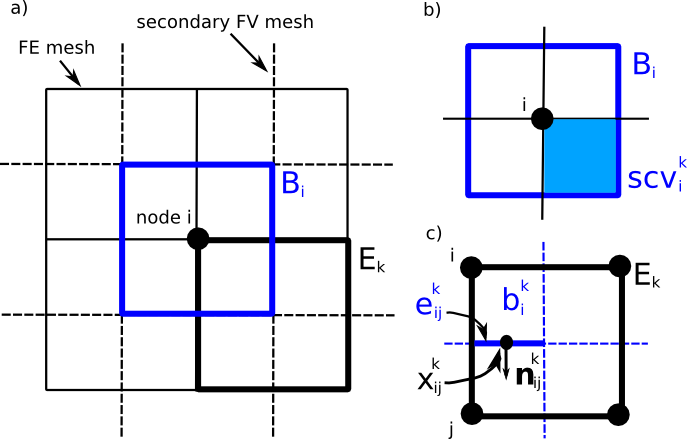
\includegraphics[width=0.8\linewidth,keepaspectratio]{png/box_disc.png}
\caption{\label{pc:box} Discretization of the box method}
\end{figure}

The FE mesh divides the box $B_i$ into subcontrolvolumes (scv's) $b^k_i$
(see Figure \ref{pc:box}b). Figure \ref{pc:box}c shows the finite element $E_k$
and the scv's $b^k_i$ inside $E_k$, which belong to four different boxes $B_i$.
Also necessary for the discretization are the faces of the subcontrolvolumes (scvf's)
$e^k_{ij}$ between the scv's $b^k_i$ and $b^k_j$, where $|e^k_{ij}|$ is the length
of the scvf. The integration points $x^k_{ij}$ on $e^k_{ij}$ and the outer normal
vector $\mathbf n^k_{ij}$ are also to be defined (see Figure \ref{pc:box}c).

The advantage of the FE method is that unstructured grids can be used, while the
FV method is mass conservative. The idea is to apply the FV method (balance of
fluxes across the interfaces) to each FV box $B_i$  and to get the fluxes across
the interfaces $e^k_{ij}$ at the integration points $x^k_{ij}$ from the FE approach.
Consequently, at each scvf the following expression results:

\begin{equation}
 	f(\tilde u(x^k_{ij})) \cdot \mathbf n^k_{ij} \: |e^k_{ij}| \qquad \textrm{with}
 	\qquad \tilde u(x^k_{ij}) = \sum_i N_i(x^k_{ij}) \cdot \hat u_i .
\end{equation}

In the following, the discretization of the balance equation is going to be derived.
From the \textsc{Reynolds} transport theorem follows the general balance equation:

\begin{equation}
	\underbrace{\int_\Omega \frac{\partial}{\partial t} \: u \: dx}_{1}
	+ \underbrace{\int_{\partial\Omega} (\mathbf{v} u + \mathbf w) \cdot \textbf n \: d\varGamma}_{2} = \underbrace{\int_\Omega q \: dx}_{3}
\end{equation}

\begin{equation}
	f(u) = \int_\Omega \frac{\partial u}{\partial t} \: dx + \int_{\Omega} \nabla \cdot
	\underbrace{\left[  \mathbf{v} u + \mathbf w(u)\right] }_{F(u)}  \: dx - \int_\Omega q \: dx = 0
\end{equation}
where term 1 describes the changes of entity $u$ within a control volume over
time, term 2 the advective, diffusive and dispersive fluxes over the interfaces
of the control volume and term 3 is the source and sink term. $\Omega$ denotes the
model domain and $F(u) = F(\mathbf v, p) = F(\mathbf v(x,t), p(x,t))$.

Like the FE method, the box method follows the principle of weighted residuals.
In the function $f(u)$ the unknown $u$ is approximated by discrete values at the
nodes of the FE mesh $\hat u_i$ and linear basis functions $N_i$ yielding an
approximate function $f(\tilde u)$. For $u\in \lbrace \mathbf v, p, x^\kappa \rbrace$
this means:

\begin{minipage}[b]{0.47\textwidth}
\begin{equation}
\label{eq:p}
	\tilde p = \sum_i N_i \hat{p}_i
\end{equation}
\begin{equation}
\label{eq:v}
	\tilde{\mathbf v} = \sum_i N_i \hat{\mathbf v}_i
\end{equation}
\begin{equation}
\label{eq:x}
	\tilde x^\kappa  = \sum_i N_i \hat x_i^\kappa
\end{equation}
\end{minipage}
\hfill
\begin{minipage}[b]{0.47\textwidth}
\begin{equation}
\label{eq:dp}
	\nabla \tilde p = \sum_i \nabla N_i \hat{p}_i
\end{equation}
\begin{equation}
\label{eq:dv}
	\nabla \tilde{\mathbf v} = \sum_i \nabla N_i \hat{\mathbf v}_i
\end{equation}
\begin{equation}
\label{eq:dx}
	\nabla \tilde x^\kappa  = \sum_i \nabla N_i \hat x_i^\kappa .
\end{equation}
\end{minipage}

Due to the approximation with node values and basis functions the differential
equations are not exactly fulfilled anymore but a residual $\varepsilon$ is produced.

\begin{equation}
	f(u) = 0  \qquad \Rightarrow \qquad f(\tilde u) = \varepsilon
\end{equation}

Application of the principle of weighted residuals, meaning the multiplication
of the residual $\varepsilon$ with a weighting function $W_j$  and claiming that
this product has to vanish within the whole domain,

\begin{equation}
	\int_\Omega W_j \cdot \varepsilon \: \overset {!}{=} \: 0 \qquad \textrm{with} \qquad \sum_j W_j =1
\end{equation}
yields the following equation:

\begin{equation}
	\int_\Omega W_j \frac{\partial \tilde u}{\partial t} \: dx + \int_\Omega W_j
	\cdot \left[ \nabla \cdot F(\tilde u) \right]  \: dx - \int_\Omega W_j
	\cdot q \: dx = \int_\Omega W_j \cdot \varepsilon \: dx \: \overset {!}{=} \: 0.	
\label{eq:weightedResidual}	
\end{equation}

For standard Galerkin schemes, the weighting functions $W_j$ are chosen the same as the ansatz functions $N_j$. However, this does not yield a locally mass-conservative scheme. 
Therefore, for the Box method, the weighting functions $W_j$ are chosen as 
the piecewise constant functions over a
control volume box $B_j$, i.e.

\begin{equation}
	W_j(x) = \begin{cases}
	          1 &x \in B_j \\
		  0 &x \notin B_j.\\
	         \end{cases}
\label{eq:weightingFunctions}	         
\end{equation}
Thus, the Box method is a Petrov-Galerkin scheme, where the weighting functions do not belong to the same function space than the ansatz functions.

Inserting definition \eqref{eq:weightingFunctions} into equation \eqref{eq:weightedResidual} and using the \textsc{Green-Gaussian} integral theorem results in
\begin{equation}
	\int_{B_j} \frac{\partial \tilde u}{\partial t} \: dx + \int_{\partial B_j}  F(\tilde u) \cdot \mathbf n \: d\varGamma_{B_j} - \int_{B_j} q \: dx  \overset {!}{=} \: 0, 	
\label{eq:BoxMassBlance}	
\end{equation}
which has to hold for every box $B_j$. 

The first term in equation \eqref{eq:BoxMassBlance} can be written as
\begin{equation}
\int_{B_j} \frac{\partial \tilde u}{\partial t} \: dx = \frac{d}{dt} \int_{B_j} \sum_i \hat u_i N_i  \: dx = \sum_i \frac{\partial \hat u_i}{\partial t} \int_{B_j}  N_i  \: dx.
\end{equation} 
Here, a mass lumping technique is applied by assuming that the storage capacity is
reduced to the nodes. This means that the integrals $M_{i,j} = \int_{B_j}  N_i \: dx$
are replaced by some mass lumped terms $M^{lump}_{i,j}$ which are defined as
\begin{equation}
	 M^{lump}_{i,j} =\begin{cases}  V_j &j = i\\
	0 &j \neq i,\\
	         \end{cases}
\end{equation}
where $V_j$ is the volume of the FV box $B_j$ associated with node $j$.
The application of this assumption yields

\begin{equation}
\label{eq:disc1}
	V_j \frac{\partial \hat u_j}{\partial t}
	+  \int_{\partial B_j}  F(\tilde u) \cdot \mathbf n \: d\varGamma_{B_j} - Q_j = 0,
\end{equation}
where $Q_j$ is an approximation (using some quadrature rule) of the integrated source/sink term $\int_{B_j} q \: dx$.

Using an implicit Euler time discretization finally
leads to the discretized form which will be applied to the mathematical
flow and transport equations:

\begin{equation}
\label{eq:discfin}
	V_j \frac{\hat u_j^{n+1} - \hat u_j^{n}}{\Delta t}
	+ \int_{\partial B_j}  F(\tilde u^{n+1}) \cdot \mathbf n
	\;  d{\varGamma}_{B_j} - Q_j^{n+1} \: = 0.
\end{equation}
Equation \eqref{eq:discfin} has to be fulfilled for each box $B_j$.

\subsection{Cell Centered Finite Volume Methods -- A Short Introduction}\label{cc}
Cell-centered finite volume methods use the elements of the grid as control volumes.
For each control volume the discrete values are determined at the element/control
volume center (not required to be the barycenters). 

We consider a domain $\Omega \subset \mathbb{R}^d$, $d \in \{ 2, 3 \}$ with boundary $\Gamma = \partial \Omega$. Within this section, we consider the following elliptic problem
\begin{equation}
  \begin{aligned}
                   \nabla \cdot \left( - \mathbf{\Lambda} \nabla u \right) &= q   &&\mathrm{in} \, \Omega \\
               \left( - \mathbf{\Lambda} \nabla u \right) \cdot \mathbf{n} &= v_N &&\mathrm{on} \, \Gamma_N \\
                                                                   u &= u_D &&\mathrm{on} \, \Gamma_D.
    \label{eq:elliptic}
  \end{aligned}
\end{equation}

Here, $\mathbf{\Lambda} = \mathbf{\Lambda}(\mathbf{x}, \mathbf{u})$ is a symmetric and positive definite tensor of second rank (e.g. permeability, diffusivity, etc.), $u = u (\mathbf{x})$ is unknown and $q = q(\mathbf{x}, \mathbf{u})$ is a source/sink. 
We denote by $\mathcal{M}$ the mesh that results from the division of the domain $\Omega$ into $n_e$ control volumes $K \subset \Omega$. Each $K$ is a polygonal open set such that $K \cap L = \emptyset, \forall{K \neq L}$ and $\overline{\Omega} = \cup_{K \in \mathcal{M}} \overline{K}$. 

For the derivation of the finite-volume formulation we integrate the first equation of \eqref{eq:elliptic} over a control volume $K$ and apply the Gauss divergence theorem:

\begin{equation}
    \int_{\partial K} \left( - \mathbf{\Lambda} \nabla u \right) \cdot \mathbf{n} \, \mathrm{d} \Gamma = \int_K q \, \mathrm{d}\Omega.
    \label{eq:ellipticIntegrated}
\end{equation}

Splitting the control volume boundary $\partial K$ into a finite number of faces $\sigma \subset \partial K$ (such that $\sigma = \overline{K} \cap \overline{L}$ for some neighboring control volume $L$) and replacing the exact fluxes by an approximation, i.e. $F_{K, \sigma} \approx \int_{\sigma} \left( - \mathbf{\Lambda} \nabla u \right) \cdot \mathbf{n} \mathrm{d} \Gamma$, yield
\begin{equation}
    \sum_{\sigma \subset \partial K} F_{K, \sigma} = Q_K, \quad \forall \, {K \in \mathcal{M}},
\label{eq:ccdisc}
\end{equation}
where $F_{K, \sigma}$ is the discrete flux through face $\sigma$ flowing out of cell $K$ and $Q_K := \int_K q \, \mathrm{d}x$ is the integrated source/sink term. Equation \eqref{eq:ccdisc} is the typical cell-centered finite-volume formulation. 
Finite-volume schemes differ in the way how the term 
$(\mathbf{\Lambda} \nabla u ) \cdot \mathbf{n} $ is approximated (i.e. the choice of the fluxes $F_{K, \sigma}$). Using the symmetry of the tensor $\mathbf{\Lambda}$, this term can be rewritten as 
$\nabla u  \cdot \mathbf{\Lambda}\mathbf{n}$, which corresponds to the directional derivative of $u$ in co-normal direction $\mathbf{\Lambda}\mathbf{n}$. 
In the following, the main ideas of the two-point flux approximation and the multi-point flux approximation methods are briefly described. Hereby, we restrict the discussion to the two-dimensional case.

Please also note that other types of equations, e.g. instationary parabolic problems, can be discretized by applying some time discretization scheme to the time derivatives and by using the finite-volume scheme for the flux discretization. For simplicity the discussion is restricted to the elliptic problem \eqref{eq:elliptic}.

\subsubsection{Tpfa Method}\label{cc_tpfa}
The linear two-point flux approximation is a simple but robust cell-centered finite-volume scheme, which is commonly used in commercial software. 
This scheme can be derived by using the conormal decomposition, which reads
\begin{equation}
\mathbf{\Lambda}_K \mathbf{n}_{K, \sigma} = t_{K,\sigma} \mathbf{d}_{K,\sigma} + \mathbf{d}^{\bot}_{K,\sigma}, \quad  t_{K,\sigma} = \frac{\mathbf{n}_{K, \sigma}^T \mathbf{\Lambda}_K \mathbf{d}_{K,\sigma} }{\mathbf{d}_{K,\sigma}^T \mathbf{d}_{K,\sigma}}, \; \mathbf{d}^{\bot}_{K,\sigma} = \mathbf{\Lambda}_K \mathbf{n}_{K, \sigma} - t_{K,\sigma} \mathbf{d}_{K,\sigma},
\label{eq:conormalDecTpfa}
\end{equation}
with the distance vector $\mathbf{d}_{K,\sigma} := \mathbf{x}_\sigma - \mathbf{x}_K$ and $\mathbf{d}_{K,\sigma}^T \mathbf{d}^{\bot}_{K,\sigma} = 0$, see Figure \ref{pc:cctpfa} for the used notations. The same can be done for the conormal $\mathbf{\Lambda}_L \mathbf{n}_{L, \sigma}$. The $t_{K,\sigma}$ and $t_{L,\sigma}$ are the transmissibilities associated with the face $\sigma$. These transmissibilities are calculated in \Dumux by using the function \texttt{computeTpfaTransmissibility}.

\begin{figure} [ht]
\centering

\includegraphics[width=0.4\linewidth,keepaspectratio]{PNG/cctpfa.png}
\caption{Two neighboring control volumes sharing the face $\sigma$.}
\label{pc:cctpfa}
\end{figure}


With these notations, it follows that for each cell $K$ and face $\sigma$ 
\begin{equation}
\nabla u \cdot \mathbf{\Lambda}_K \mathbf{n}_{K, \sigma} =  t_{K,\sigma} \nabla u \cdot \mathbf{d}_{K,\sigma} + \nabla u \cdot \mathbf{d}^{\bot}_{K,\sigma}.
\end{equation}
For the Tpfa scheme, the second part in the above equation is neglected. By using the fact that $\nabla u \cdot \mathbf{d}_{K,\sigma} \approx u_\sigma - u_K$, the discrete fluxes for face $\sigma$ are given by
\begin{equation}
F_{K,\sigma} = -\meas{\sigma}  t_{K,\sigma} (u_\sigma - u_K), \qquad F_{L,\sigma} = -\meas{\sigma}  t_{L,\sigma} (u_\sigma - u_L).
\label{eq:TPFAOneSided}
\end{equation}
Enforcing local flux conservation, i.e. $F_{K,\sigma}+F_{L,\sigma}=0$, results in 
\begin{equation}
u_\sigma = \frac{t_{K,\sigma} u_K + t_{L,\sigma} u_L}{t_{K,\sigma}  + t_{L,\sigma}}.
\end{equation}
With this, the fluxes \eqref{eq:TPFAOneSided} are rewritten as
\begin{equation}
F_{K,\sigma} = \meas{\sigma}  \frac{t_{K,\sigma} t_{L,\sigma}}{t_{K,\sigma} + t_{L,\sigma}} (u_K - u_L), \quad F_{L,\sigma} = \meas{\sigma}  \frac{t_{K,\sigma} t_{L,\sigma}}{t_{K,\sigma} + t_{L,\sigma}} (u_L - u_K).
\label{eq:TPFAFlux}
\end{equation}
By neglecting the orthogonal term, the consistency of the scheme is lost for general grids, where $\nabla u \cdot \mathbf{d}^{\bot}_{K,\sigma} \not = 0$. The consistency is achieved only for so-called K-orthogonal grids for which $\mathbf{d}^{\bot}_{K,\sigma} = 0$. For such grids we deduce that 
\begin{equation}
\frac{t_{K,\sigma} t_{L,\sigma}}{t_{K,\sigma} + t_{L,\sigma}} = \frac{\tau_{K,\sigma} \tau_{L,\sigma}}{\tau_{K,\sigma} d_{L,\sigma} + \tau_{L,\sigma} d_{K,\sigma}},
\label{eq:TPFAcoeffNew}
\end{equation}
with $\tau_{K,\sigma} := \mathbf{n}_{K, \sigma} \mathbf{\Lambda}_K\mathbf{n}_{K, \sigma}, \tau_{L,\sigma} := \mathbf{n}_{L, \sigma} \mathbf{\Lambda}_L\mathbf{n}_{L, \sigma}$, $d_{K,\sigma}:= \mathbf{n}_{K, \sigma} \cdot \mathbf{d}_{K, \sigma}$, and $d_{L,\sigma}:= \mathbf{n}_{L, \sigma} \cdot \mathbf{d}_{L, \sigma}$. This reduces, for the case of scalar permeability, to a distance weighted harmonic averaging of permeabilities.

 

\subsubsection{Mpfa Method}\label{cc_mpfa}
Expressions for the face fluxes $F_{K, \sigma}$ are usually obtained by introducing intermediate face unknowns $u_\sigma$ in addition to the cell unknowns $u_K$ and enforcing the physically motivated continuity of fluxes and continuity of the solution across the faces. For a face $\sigma$ between the two polygons $K$ and $L$ these conditions read:
\begin{equation}
    \begin{aligned}
        &F_{K, \sigma} + F_{L, \sigma} = 0 \\
        &{u}_{K,\sigma} = {u}_{L,\sigma} = {u}_{\sigma}.
        \label{eq:sigmaConditions}
    \end{aligned}
\end{equation}
Using these conditions the intermediate face unknowns ${u}_\sigma$ can be eliminated and the fluxes are expressed as a function of the cell unknowns $u_N$ and associated transmissibilities $t^N_{K,\sigma}$:

\begin{equation}
    F_{K,\sigma} = \sum_{N \in \mathcal{S}_{K,\sigma}} t^N_{K,\sigma} u_{N}.
    \label{eq:FVFluxExpression}
\end{equation}

\begin{figure} [ht]
\centering
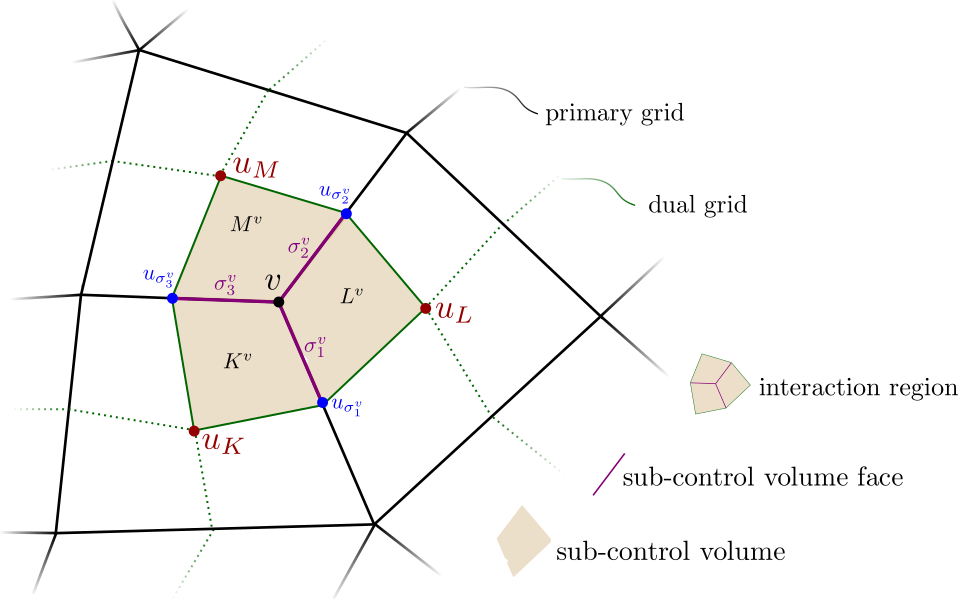
\includegraphics[width=0.8\linewidth,keepaspectratio]{PNG/mpfa_iv.png}
\caption{Interaction region for the Mpfa-O method. The graphic on the right illustrates how the sub-control volume $L^v$ and face $\sigma^v_2$ are embedded in cell $L$. Note that the face stencils for all sub-control volume faces in the depicted interaction region are $\mathcal{S}_{\sigma^v_i} = \{ K,L,M \}$, meaning that the fluxes over the sub-control volume faces depend on the three cell unknowns $u_K, u_L, u_M$.}
\label{pc:interactionRegion_mpfa}
\end{figure}

The main difference between the various finite-volume schemes available is the assembly of the face fluxes, i.e. the computation of the $t^N_{K,\sigma}$ and the size of $\mathcal{S}_{K,\sigma}$. For the Tpfa, that has been presented in the last section, the stencil and transmissibilities are given as
\begin{equation*}
\mathcal{S}_{K,\sigma} = \lbrace K,L \rbrace, \quad t^K_{K,\sigma} =  \meas{\sigma}  \frac{t_{K,\sigma} t_{L,\sigma}}{t_{K,\sigma} + t_{L,\sigma}},\; t^L_{K,\sigma} =  -\meas{\sigma}  \frac{t_{K,\sigma} t_{L,\sigma}}{t_{K,\sigma} + t_{L,\sigma}},
\end{equation*}
with $t_{K,\sigma},t_{L,\sigma}$ as defined in equation \eqref{eq:conormalDecTpfa}.

In the following, a multi-point flux approximation method (Mpfa-O method), which was first introduced in \citet{Aavatsmark2002}, is presented. The main difference to the Tpfa scheme is the fact that a consistent discrete gradient is constructed, i.e. the term $\nabla u \cdot \mathbf{d}^{\bot}_{K,\sigma}$ is not neglected.

For this scheme, a dual grid is created by connecting the barycenters of the cells with the barycenters of the faces ($d=2$) or the barycenters of the faces and edges ($d=3$). This divides each cell into sub-control volumes $K^v$. Analogously, each face is sub-divided into sub-control volume faces $\sigma^v$, see Figure \ref{pc:interactionRegion_mpfa}. We allow for piecewise constant $\mathbf{\Lambda}$ (per cell) and construct discrete gradients $\nabla_\mathcal{D}^{K^v} u$ (per sub-control volume $K^v$). 
In the following, we restrict our discussion to the two-dimensional setup that is shown in Figure \ref{pc:interactionRegion_mpfa}.  
Here, the discrete gradients are constructed to be consistent such that the following conditions hold:
\begin{equation}
\nabla_\mathcal{D}^{K^v} u \cdot (\mathbf{x}_{\sigma^v_1}- \mathbf{x}_{K}) = u_{\sigma^v_1} - u_K, \quad \nabla_\mathcal{D}^{K^v} u \cdot (\mathbf{x}_{\sigma^v_3}- \mathbf{x}_{K}) = u_{\sigma^v_3} - u_K.
\end{equation}
Thus, a discrete gradient (for sub-control volume $K^v$) that fulfills  these conditions is given as
\begin{equation}
\nabla_\mathcal{D}^{K^v} u  = \mathbb{D}^{-T}_{K^v}
 \begin{bmatrix}
  u_{\sigma^v_1} - u_K \\
  u_{\sigma^v_3} - u_K
 \end{bmatrix}, \qquad \text{ with }\; \mathbb{D}_{K^v} := 
  \begin{bmatrix}
   \mathbf{x}_{\sigma^v_1}- \mathbf{x}_K & \mathbf{x}_{\sigma^v_3} - \mathbf{x}_K
 \end{bmatrix}.
 \label{eq:MPFAGradientRecons}
\end{equation}

This enables us to write the discrete flux across $\sigma^v_1$ from cell $K$ as follows:
\begin{equation}
    F_{K, \sigma^v_1} := - |\sigma^v_1| \mathbf{n}_{\sigma^v_1}^T \mathbf{\Lambda}_K \nabla_\mathcal{D}^{K^v} u.
    \label{eq:discreteFlux}
\end{equation}
Inserting the discrete gradient, yields
\begin{equation}
    F_{K, \sigma^v_1} = \omega_{K,\sigma^v_1\sigma^v_1}(u_K - u_{\sigma^v_1}) + \omega_{K,\sigma^v_1 \sigma^v_3}(u_K - u_{\sigma^v_3}),
    \label{eq:discreteFluxRef}
\end{equation}
with $(\omega_{K,\sigma^v_1\sigma^v_1},\omega_{K,\sigma^v_1 \sigma^v_3})^T = |\sigma^v_1| \mathbb{D}^{-1}_{K^v}\mathbf{\Lambda}_K \mathbf{n}_{\sigma^v_1}$. 
\\ \ \\
To deduce a cell-centered scheme, the introduced face unknowns $u_{\sigma^v_i}$ have to be eliminated. This is done by enforcing flux continuity for each sub-control volume face, i.e.
\begin{align}
F_{K, \sigma^v_1} + F_{L, \sigma^v_1} &= 0, \\ F_{K, \sigma^v_3} + F_{M, \sigma^v_3} &= 0, \\ F_{L, \sigma^v_2} + F_{M, \sigma^v_2} &= 0.
\end{align}
This results in a system of equations for the face unknowns $\mathbf{u}_{\sigma}$
\begin{equation}
\mathbb{A}^{3\times 3} \mathbf{u}_{\sigma} = \mathbb{B}^{3\times 3} \mathbf{u},
\end{equation}
where $\mathbf{u}$ contains the three cell unknowns $u_K,u_L,u_M$ and $\mathbf{u}_{\sigma}$ the three face unknowns $u_{\sigma^v_1}, u_{\sigma^v_2}, u_{\sigma^v_3}$. 
Inserting these face unknowns into the flux expression \eqref{eq:discreteFluxRef} yields
\begin{equation}
    F_{K,\sigma^v_i} = \sum_{N \in \lbrace K,L,M \rbrace } t^N_{K,\sigma^v_i} u_{N} = \mathbf{t}_{K,\sigma^v_i} \cdot \mathbf{u},
    \label{eq:FVFluxExpressionSubFace}
\end{equation}
for each cell $K$ and sub-control volume face $\sigma^v_i$. 
In \Dumux the transmissibility vector $\mathbf{t}_{K,\sigma^v_i}$ is returned by the function \texttt{advectionTijSecondaryIv()} or \texttt{advectionTijPrimaryIv()}, depending on the chosen interaction volume type (the primary interaction volume is used by default).

% \subsubsection{NLTPFA}\label{cc_nltpfa}
% TODO

\subsection{Staggered Grid -- A Short Introduction}\label{staggered}

\begin{figure}[ht]
\centering
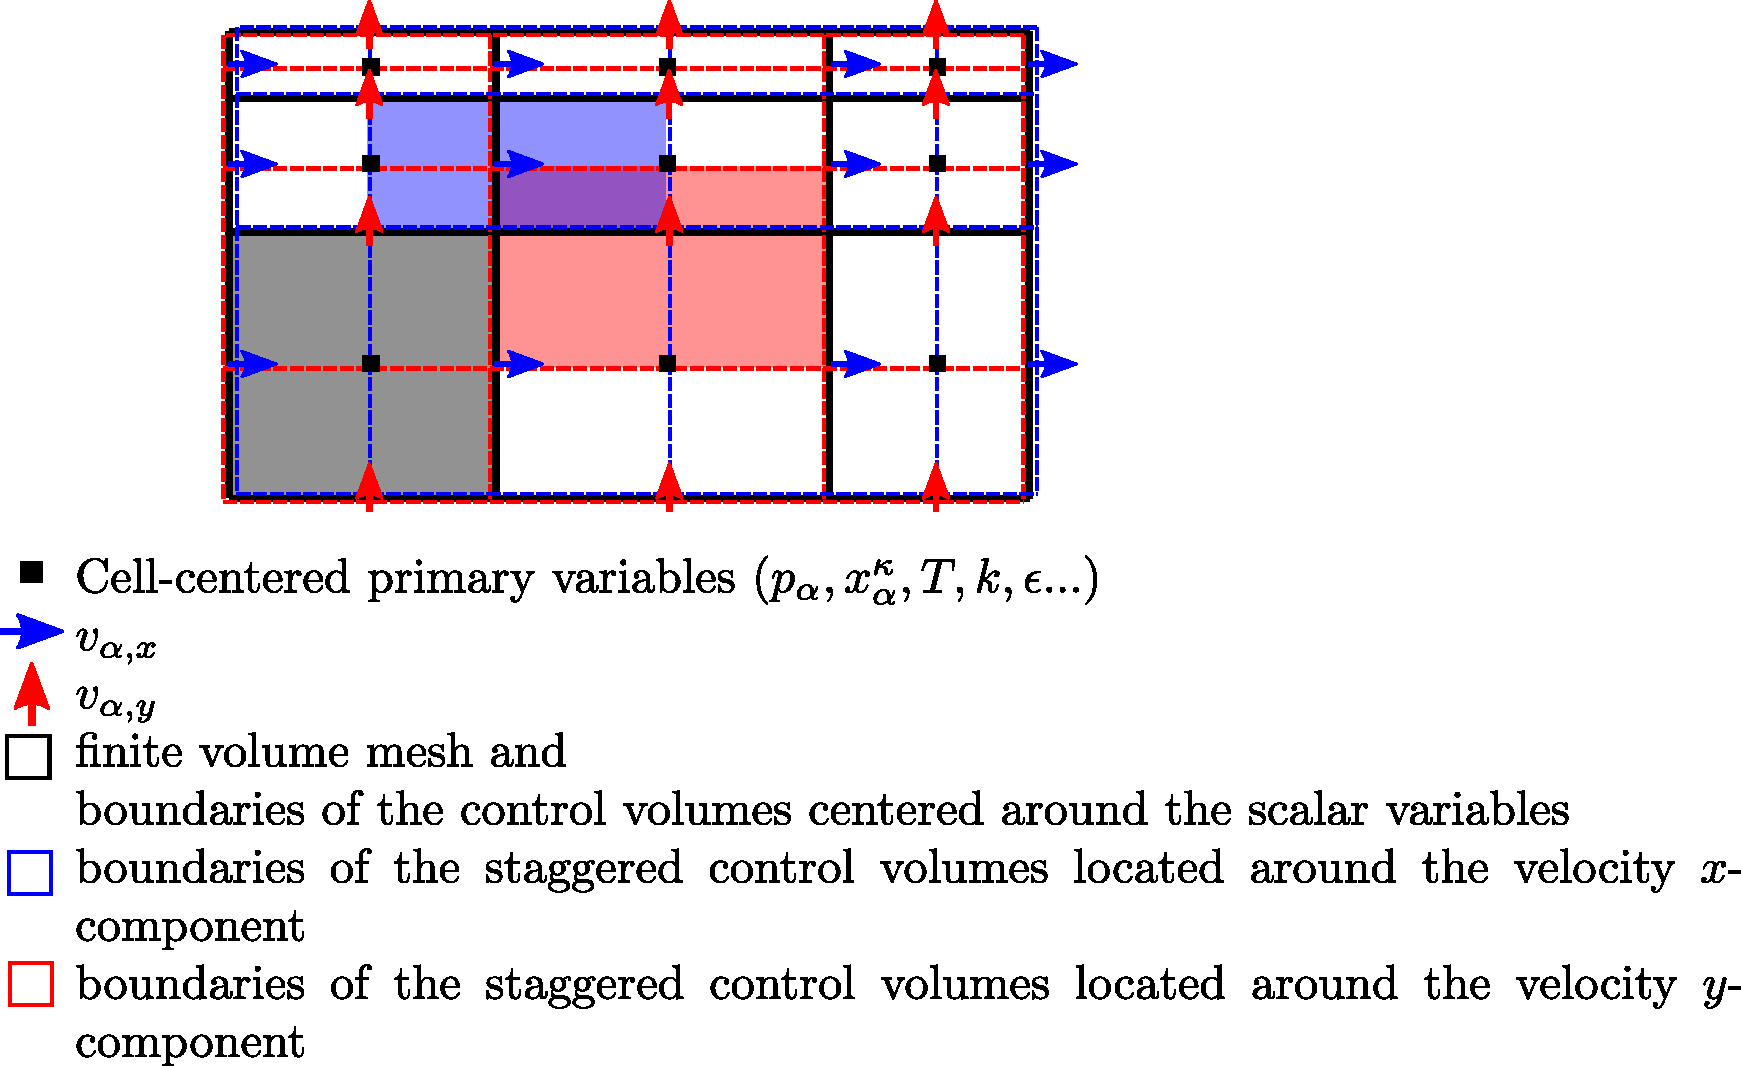
\includegraphics[width=.8\linewidth]{./pdf/staggered_grid.pdf}
\caption{\label{pc:staggered} Discretization of the staggered-grid method. The figure shows the different control volume arrangements, which are staggered with respect to each other. There are the control volumes centered around the scalar primary variables in black, the control volumes located around the $x$-component of the velocity in blue and the control volumes located around the $y$-components of the velocity in red. The control volume boundaries are given by lines. Additionally, there is one shaded example control volume each.\\
In the two-dimensional free-flow models, the continuity equation is discretized using the black control volumes, the $x$-component of the momentum equation is discretized using the blue control volumes and the $y$-component is discretized using the red control volumes. In three dimensions this works analogously.}
\end{figure}

The staggered-grid or marker-and-cell method uses a finite volume method with different control volumes for different equations. There are control volumes centered around the scalar primary variables. They correspond to the finite volume mesh. Additionally, there are control volumes located around the $x,y$ and (in 3D) $z$ velocity components which are shifted in the $x,y$ and $z$ direction, such that the velocity components are located on the edges of the cell-centered finite volume mesh (see Figure~\ref{pc:staggered}). As for the cell-centered method, the fluxes are evaluated at the edges of each control volume with a two-point flux approximation, cf. \ref{cc}.\par
The staggered-grid method is robust, mass conservative, and free of pressure oscillations
but should, as the cell-centered TPFA method, only be applied for structured grids.
Currently, all free-flow models in \Dumux use the staggered-grid discretization.

\section{Steps of a \Dumux Simulation}
\label{flow}


This chapter is supposed to give a short overview over how things are ``handed around'' in \Dumux. It
is not a comprehenisve guide through the modeling framework of \Dumux, but
hopefully it will help getting to grips with it.

In Section \ref{content} the structure of \Dumux is shown from a \emph{content}
point of view.

\subsection{Structure -- by Content}

\label{content}
In Figure \ref{fig:algorithm}, the algorithmic representations of a monolithical
solution solution scheme is illustrated down to the element level.

\begin{figure}[hbt]
\setcounter{thingCounter}{0}

\scriptsize
\sffamily
\begin{center}\parbox{0cm}{
\begin{tabbing}
\textbf{{\begin{turn}{45}\color{black}\numberThis{main}{init}\end{turn}}}             \=
\textbf{{\begin{turn}{45}\color{dumuxBlue}\numberThis{time step}{prep}\end{turn}}}            \=
\textbf{{\begin{turn}{45}\color{Mulberry}\numberThis{\textsc{Newton}}{elem}\end{turn}}}         \=
\textbf{{\begin{turn}{45}\color{dumuxYellow}\numberThis{element}{calc}\end{turn}}}             \=  \\
\\
\color{black}initialize \\
\color{black}\textbf{foreach} time step\\

  \> \color{dumuxBlue}\textbf{foreach} \textsc{Newton} iteration \\

    \> \> \color{Mulberry}\textbf{foreach} element \\

      \> \> \> \color{dumuxYellow}- calculate element \\
      \> \> \> \color{dumuxYellow}\; residual vector and \\
      \> \> \> \color{dumuxYellow}\; Jacobian matrix\\
      \> \> \> \color{dumuxYellow}- assemble into global\\
      \> \> \> \color{dumuxYellow}\; residual vector and \\
      \> \> \> \color{dumuxYellow}\;{Jacobian} matrix \\

    \> \> \color{Mulberry}\textbf{endfor} \\

    \> \> \color{Mulberry}solve linear system\\
    \> \> \color{Mulberry}update solution\\
    \> \> \color{Mulberry}check for \textsc{Newton} convergence\\
  \> \color{dumuxBlue}\textbf{endfor}\\
  \> \color{dumuxBlue}- adapt time step size, \\
  \> \color{dumuxBlue}\; possibly redo with smaller step size\\
  \> \color{dumuxBlue}- write result\\
\color{black}\textbf{endfor}\\
\color{black}finalize
\end{tabbing}}
\end{center}
\caption{Structure of a monolithical solution scheme in \Dumux.}
\label{fig:algorithm}
\end{figure}

\subsection{Structure -- by Implementation}
A possible starting point to understand how the abovementioned algorithm is implemented within \Dumux,
is the example main file
\url{https://git.iws.uni-stuttgart.de/dumux-repositories/dumux-course/releases/3.0/exercises/exercise-mainfile/exercise_1p_a.cc}

\section{Property System}
\label{sec:propertysystem}
A high level overview over the property system's design and principle ideas
are given, then follows a reference and a self-contained example.

\subsection{Motivation and features}
The \Dumux property system was designed as an attempt to mitigate the
problems of traits classes. It can be seen as a traits system
which allows easy inheritance and any acyclic dependency of parameter
definitions. Just like traits, the \Dumux property system is a compile
time mechanism, thus there is no run-time performance penalty associated
with it.

In the context of the \Dumux property system, a property is an arbitrary
class body which may contain type definitions, values and methods. Each
property has a so-called \emph{property tag} which labels its name.

Just like normal classes, properties can be arranged in hierarchies. In
the context of the \Dumux property system, nodes of the inheritance
hierarchy are called \emph{type tags}.

It also supports \emph{property nesting} and
\emph{introspection}. Property nesting means that the definition of
a property can depend on the value of other properties which may be
defined for arbitrary levels of the inheritance hierarchy. The term
introspection denotes the ability to generate diagnostic messages
which can be used to find out where a certain property was defined and
how it was inherited.

\subsection{How-to}
All source files which use the property system should include
the header file \path{dumux/common/propertysystem.hh}.
Declaration of type tags and
property tags as well as defining properties must be done inside the
namespace \texttt{Dumux::Properties}.

\subsubsection{Defining Type Tags}
New nodes in the type tag hierarchy can be defined using
\begin{lstlisting}[style=DumuxCode]
NEW_TYPE_TAG(NewTypeTagName, INHERITS_FROM(BaseTagName1, BaseTagName2, ...));
\end{lstlisting}
where the \texttt{INHERITS\_FROM} part is optional. To avoid
inconsistencies in the hierarchy, each type tag may be defined only
once for a program.

\vskip1ex\noindent
Example:
\begin{lstlisting}[style=DumuxCode]
namespace Dumux {
namespace Properties {
NEW_TYPE_TAG(MyBaseTypeTag1);
NEW_TYPE_TAG(MyBaseTypeTag2);

NEW_TYPE_TAG(MyDerivedTypeTag, INHERITS_FROM(MyBaseTypeTag1, MyBaseTypeTag2));
}}
\end{lstlisting}

\subsubsection{Declaring Property Tags}
New property tags, i.e. labels for properties, are declared
using
\begin{lstlisting}[style=DumuxCode]
NEW_PROP_TAG(NewPropTagName);
\end{lstlisting}
A property tag can be declared arbitrarily often, in fact it is
recommended that all properties are declared in each file where they
are used.

\vskip1ex\noindent
Example:
\begin{lstlisting}[style=DumuxCode]
namespace Dumux {
namespace Properties {
NEW_PROP_TAG(MyPropertyTag);
}}
\end{lstlisting}

\subsubsection{Defining Properties}
The value of a property on a given node of the type tag hierarchy is
defined using
\begin{lstlisting}[style=DumuxCode]
SET_PROP(TypeTagName, PropertyTagName)
{
  // arbitrary body of a struct
};
\end{lstlisting}
For each program, a property itself can be declared at most once,
although properties may be overwritten for derived type tags.

Also, the following convenience macros are available to define simple
properties:
\begin{lstlisting}[style=DumuxCode]
SET_TYPE_PROP(TypeTagName, PropertyTagName, type);
SET_BOOL_PROP(TypeTagName, PropertyTagName, booleanValue);
SET_INT_PROP(TypeTagName, PropertyTagName, integerValue);
SET_SCALAR_PROP(TypeTagName, PropertyTagName, floatingPointValue);
\end{lstlisting}

\vskip1ex\noindent
Example:
\begin{lstlisting}[style=DumuxCode]
namespace Dumux {
namespace Properties {
NEW_TYPE_TAG(MyTypeTag);

NEW_PROP_TAG(MyCustomProperty);
NEW_PROP_TAG(MyType);

NEW_PROP_TAG(MyBoolValue);
NEW_PROP_TAG(MyIntValue);
NEW_PROP_TAG(MyScalarValue);

SET_PROP(MyTypeTag, MyCustomProperty)
{
  static void print() { std::cout << "Hello, World!\n"; }
};
SET_TYPE_PROP(MyTypeTag, MyType, unsigned int);

SET_BOOL_PROP(MyTypeTag, MyBoolValue, true);
SET_INT_PROP(MyTypeTag, MyIntValue, 12345);
SET_SCALAR_PROP(MyTypeTag, MyScalarValue, 12345.67890);
}}
\end{lstlisting}

\subsubsection{Un-setting Properties}
Sometimes an inherited properties do not make sense for a certain
node in the type tag hierarchy. These properties can be explicitly
un-set using
\begin{lstlisting}[style=DumuxCode]
UNSET_PROP(TypeTagName, PropertyTagName);
\end{lstlisting}
The un-set property can not be set for the same type tag, but of
course derived type tags may set it again.

\vskip1ex\noindent
Example:
\begin{lstlisting}[style=DumuxCode]
namespace Dumux {
namespace Properties {
NEW_TYPE_TAG(BaseTypeTag);
NEW_TYPE_TAG(DerivedTypeTag, INHERITS_FROM(BaseTypeTag));

NEW_PROP_TAG(TestProp);

SET_TYPE_PROP(BaseTypeTag, TestProp, int);
UNSET_PROP(DerivedTypeTag, TestProp);
// trying to access the 'TestProp' property for 'DerivedTypeTag'
// will trigger a compiler error!
}}
\end{lstlisting}

\subsubsection{Converting Tag Names to Tag Types}
For the \Cplusplus compiler, property and type tags are like ordinary
types. Both can thus be used as template arguments. To convert a
property tag name or a type tag name into the corresponding type, the
macros \texttt{TTAG(TypeTagName)} and \texttt{PTAG(PropertyTagName)}
ought to be used.

\subsubsection{Retrieving Property Values}
The value of a property can be retrieved using
\begin{lstlisting}[style=DumuxCode]
GET_PROP(TypeTag, PropertyTag)
\end{lstlisting}
or using the convenience macros
\begin{lstlisting}[style=DumuxCode]
GET_PROP_TYPE(TypeTag, PropertyTag)
GET_PROP_VALUE(TypeTag, PropertyTag)
\end{lstlisting}

\vskip1ex
\noindent
The first convenience macro retrieves the type defined using
\texttt{SET\_TYPE\_PROP} and is equivalent to
\begin{lstlisting}[style=DumuxCode]
GET_PROP(TypeTag, PropertyTag)::type
\end{lstlisting}
while the second convenience macro retrieves the value of any property
defined using one of the macros \texttt{SET\_}$\{$\texttt{INT,BOOL,SCALAR}$\}$\texttt{\_PROP} and is
equivalent to
\begin{lstlisting}[style=DumuxCode]
GET_PROP(TypeTag, PropertyTag)::value
\end{lstlisting}

\vskip1ex\noindent
Example:\nolinebreak
\begin{lstlisting}[style=DumuxCode]
template <TypeTag>
class MyClass {
  // retrieve the ::value attribute of the 'NumEq' property
  enum { numEq = GET_PROP(TypeTag, NumEq)::value };
  // retrieve the ::value attribute of the 'NumPhases' property using the convenience macro
  enum { numPhases = GET_PROP_VALUE(TypeTag, NumPhases) };

  // retrieve the ::type attribute of the 'Scalar' property
  typedef typename GET_PROP(TypeTag, Scalar)::type Scalar;
  // retrieve the ::type attribute of the 'Vector' property using the convenience macro
  typedef typename GET_PROP_TYPE(TypeTag, Vector) Vector;
};
\end{lstlisting}

\subsubsection{Nesting Property Definitions}
Inside property definitions there is access to all other properties
which are defined somewhere on the type tag hierarchy. The node for
which the current property is requested is available via the keyword
\texttt{TypeTag}. Inside property class bodies this can be used to
retrieve other properties using the \texttt{GET\_PROP} macros.

\vskip1ex\noindent
Example:
\begin{lstlisting}[style=DumuxCode]
SET_PROP(MyModelTypeTag, Vector)
{
private: typedef typename GET_PROP_TYPE(TypeTag, Scalar) Scalar;
public: typedef std::vector<Scalar> type;
};
\end{lstlisting}

\subsection{A Self-Contained Example}
As a concrete example, let us consider some kinds of cars: Compact
cars, sedans, trucks, pickups, military tanks and the Hummer-H1 sports
utility vehicle. Since all these cars share some characteristics, it
makes sense to inherit those from the closest matching car type and
only specify the properties which are different. Thus, an inheritance
diagram for the car types above might look like outlined in Figure
\ref{fig:car-hierarchy}.

\begin{figure}[t]
  \centering
  \subfloat[]{
    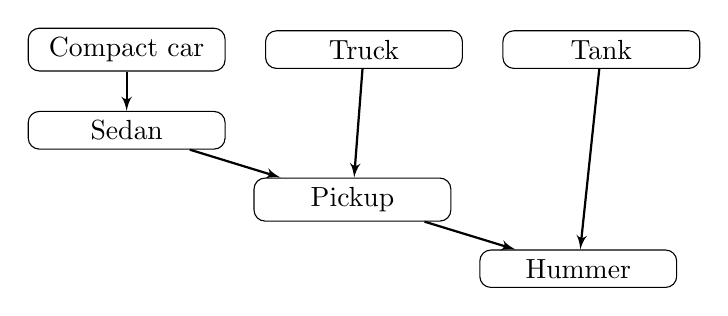
\begin{tikzpicture}
      [cars/.style={rectangle,draw=black,rounded corners,minimum width=2.5cm,node distance=0.5cm}]
      % place nodes
      \node[cars] (compact) {Compact car};
      \node[cars] (sedan) [below=of compact] {Sedan};
      \node[cars] (truck) [right=of compact] {Truck};
      \node[cars] (pickup) [below right= of sedan] {Pickup};
      \node[cars] (tank) [right=of truck] {Tank};
      \node[cars] (hummer) [below right= of pickup] {Hummer};
      % add edges
      \draw [-latex',thick] (compact) -- (sedan);
      \draw [-latex',thick] (sedan) -- (pickup);
      \draw [-latex',thick] (truck) -- (pickup);
      \draw [-latex',thick] (tank) -- (hummer);
      \draw [-latex',thick] (pickup) -- (hummer);
    \end{tikzpicture}
    \label{fig:car-hierarchy}
  }
  \hspace*{0.5cm}
  \subfloat[]{
    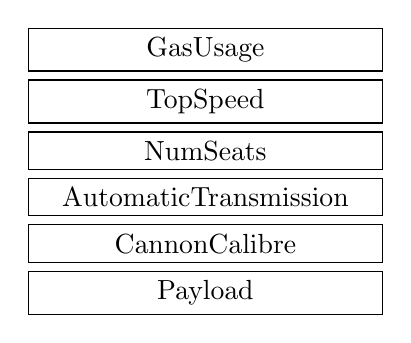
\begin{tikzpicture}
      [propertyBox/.style={rectangle,draw=black,minimum width=4.5cm,node distance=0.1cm}]
      \node[propertyBox] (gasUsage) {GasUsage};
      \node[propertyBox] (speed) [below=of gasUsage] {TopSpeed};
      \node[propertyBox] (seats) [below=of speed] {NumSeats};
      \node[propertyBox] (automatic) [below=of seats] {AutomaticTransmission};
      \node[propertyBox] (calibre) [below=of automatic] {CannonCalibre};
      \node[propertyBox] (payload) [below=of calibre] {Payload};
    \end{tikzpicture}
    \label{fig:car-propertynames}
  }
  \caption{\textbf{(a)}~A possible property inheritance graph for
    various kinds of cars.  The lower nodes inherit from higher ones;
    Inherited properties from nodes on the right take precedence over the
    properties defined on the left. \textbf{(b)}~Property names
    which make sense for at least one of the car types of (a).}
\end{figure}

Using the \Dumux property system, this inheritance hierarchy is
defined by:
\begin{lstlisting}[name=propsyscars,style=DumuxCode]
#include <dumux/common/propertysystem.hh>
#include <iostream>

namespace Dumux {
namespace Properties {
NEW_TYPE_TAG(CompactCar);
NEW_TYPE_TAG(Truck);
NEW_TYPE_TAG(Tank);
NEW_TYPE_TAG(Sedan, INHERITS_FROM(CompactCar));
NEW_TYPE_TAG(Pickup, INHERITS_FROM(Sedan, Truck));
NEW_TYPE_TAG(HummerH1, INHERITS_FROM(Pickup, Tank));
\end{lstlisting}

Figure \ref{fig:car-propertynames} lists a few property names which
make sense for at least one of the nodes of Figure
\ref{fig:car-hierarchy}. These property names can be declared as
follows:
\begin{lstlisting}[name=propsyscars,style=DumuxCode]
NEW_PROP_TAG(TopSpeed); // [km/h]
NEW_PROP_TAG(NumSeats); // []
NEW_PROP_TAG(CanonCaliber); // [mm]
NEW_PROP_TAG(GasUsage); // [l/100km]
NEW_PROP_TAG(AutomaticTransmission); // true/false
NEW_PROP_TAG(Payload); // [t]
\end{lstlisting}

\noindent
So far, the inheritance hierarchy and the property names are completely
separate. What is missing is setting some values for the property
names on specific nodes of the inheritance hierarchy. Let us assume
the following:
\begin{itemize}
\item For a compact car, the top speed is the gas usage in $\unitfrac{l}{100km}$
  times $30$, the number of seats is $5$ and the gas usage is
  $\unitfrac[4]{l}{100km}$.
\item A truck is by law limited to $\unitfrac[100]{km}{h}$ top speed, the number
  of seats is $2$, it uses $\unitfrac[18]{l}{100km}$ and has a cargo payload of
  $\unit[35]{t}$.
\item A tank exhibits a top speed of $\unitfrac[60]{km}{h}$, uses $\unitfrac[65]{l}{100km}$
  and features a $\unit[120]{mm}$ diameter canon
\item A sedan has a gas usage of $\unitfrac[7]{l}{100km}$, as well as an automatic
  transmission, in every other aspect it is like a compact car.
\item A pick-up truck has a top speed of $\unitfrac[120]{km}{h}$ and a payload of
  $\unit[5]{t}$. In every other aspect it is like a sedan or a truck but if in
  doubt, it is more like a truck.
\item The Hummer-H1 SUV exhibits the same top speed as a pick-up
  truck.  In all other aspects it is similar to a pickup and a tank,
  but, if in doubt, more like a tank.
\end{itemize}

\noindent
Using the \Dumux property system, these assumptions are formulated
using
\begin{lstlisting}[name=propsyscars,style=DumuxCode]
SET_INT_PROP(CompactCar, TopSpeed, GET_PROP_VALUE(TypeTag, GasUsage) * 30);
SET_INT_PROP(CompactCar, NumSeats, 5);
SET_INT_PROP(CompactCar, GasUsage, 4);

SET_INT_PROP(Truck, TopSpeed, 100);
SET_INT_PROP(Truck, NumSeats, 2);
SET_INT_PROP(Truck, GasUsage, 18);
SET_INT_PROP(Truck, Payload, 35);

SET_INT_PROP(Tank, TopSpeed, 60);
SET_INT_PROP(Tank, GasUsage, 65);
SET_INT_PROP(Tank, CanonCaliber, 120);

SET_INT_PROP(Sedan, GasUsage, 7);
SET_BOOL_PROP(Sedan, AutomaticTransmission, true);

SET_INT_PROP(Pickup, TopSpeed, 120);
SET_INT_PROP(Pickup, Payload, 5);

SET_INT_PROP(HummerH1, TopSpeed, GET_PROP_VALUE(TTAG(Pickup), TopSpeed));
\end{lstlisting}

\noindent
At this point, the Hummer-H1 has a $\unit[120]{mm}$ canon which it inherited
from its military ancestor. It can be removed by
\begin{lstlisting}[name=propsyscars,style=DumuxCode]
UNSET_PROP(HummerH1, CanonCaliber);

}} // close namespaces
\end{lstlisting}

\noindent
Now property values can be retrieved and some diagnostic messages can
be generated. For example
\begin{lstlisting}[name=propsyscars,style=DumuxCode]
int main()
{
    std::cout << "top speed of sedan: " << GET_PROP_VALUE(TTAG(Sedan), TopSpeed) << "\n";
    std::cout << "top speed of truck: " << GET_PROP_VALUE(TTAG(Truck), TopSpeed) << "\n";

    std::cout << PROP_DIAGNOSTIC(TTAG(Sedan), TopSpeed);
    std::cout << PROP_DIAGNOSTIC(TTAG(HummerH1), CanonCaliber);

    Dumux::Properties::print<TTAG(Sedan)>();
}
\end{lstlisting}
will yield the following output:
\begin{lstlisting}[style=Bash, basicstyle=\ttfamily\scriptsize\let\textcolor\textcolordummy]
$ top speed of sedan: 210
$ top speed of truck: 100
$ Properties for Sedan:
$   bool   AutomaticTransmission = 'true' defined at test_propertysystem.cc:68
$   int    GasUsage = '7' defined at test_propertysystem.cc:67
$   Inherited from CompactCar:
$     int    NumSeats = '5' defined at test_propertysystem.cc:55
$     int    TopSpeed = '::Dumux::Properties::GetProperty<TypeTag, ::Dumux::Properties::PTag::GasUsage>::p::value * 30' defined at test_propertysystem.cc:54
\end{lstlisting}

\subsection{Property and Parameter Values}
In \Dumux three different ways to obtain the value of a property are available:
\begin{description}
\item[\texttt{{\small GET\_PROP\_VALUE:}}]
Always returns the \emph{compile-time} specified value of the property. This is
needed for properties, which are not intended to be changed by parameter files.

\item[\texttt{{\small GET\_PARAM\_FROM\_GROUP:}}]
Returns the compile-time specified value, if this value is not be overwritten
by the parameter input file.

\item[\texttt{{\small GET\_RUNTIME\_PARAM\_FROM\_GROUP:}}]
Always returns a \emph{run-time} specified value. If the value is not specified
at run-time an error is thrown. This is needed for problem specific properties
or properties, which do not have a meaningful default value.
\end{description}

\section{Grid Handling}
\label{sec:gridhandling}

This section summarizes some ideas about grid generation and grid formats that can be used by \Dumux. In general,
\Dumux can read grids from file, or, construct grids inside the code. All grids are constructed inside a so called \texttt{GridCreator} which is a \Dumux property.
Note that some \texttt{GridCreator}s are already available in \Dumux, so e.g.
construction of a structured grid is fairly easy. We will subsequently introduce the supported file formats, the standard grid creator and its capabilities,
and briefly mention how to customize and deal with common other grid formats.

\subsection{Supported file formats}
\Dumux can read grids from file using the Dune Grid Format (DGF) or the Gmsh mesh format.

\subsubsection{Dune Grid Format}
Most of our \Dumux tests and tutorials use the Dune Grid Format (DGF) to read in grids. A detailed description
of the DGF format and some examples can be found in the \Dune doxygen documentation
\textbf{(Modules $\rightarrow$ I/O $\rightarrow$ Dune Grid Format (DGF)}). To generate larger or more
complex DGF files, we recommend to write your own scripts, e.g in \Cplusplus, Matlab or Python.

The DGF format can also used to read in spatial parameters defined on the grid. These parameters can
be defined on nodes as well as on the elements. An example for predefined parameters on a grid is
the \texttt{test\_boxco2} or \texttt{test\_cco2} in the  \texttt{dumux/test/porousmediumflow/co2/implicit/} folder.

\subsubsection{Gmsh Mesh Format}
Gmsh is an open-source flexible grid generator for unstructured finite-element meshes (\cite{GEUZAINE2009}, \url{http://geuz.org/gmsh/}).
\Dumux supports the default Gmsh mesh format (MSH). For the format specifics and how to create grids with Gmsh, e.g. using
the provided GUI, we refer to the Gmsh documentation (\url{http://geuz.org/gmsh/doc/texinfo/gmsh.html}).

The MSH format can contain element and boundary markers defined in the grid. Thus, boundaries can be easily marked as e.g. inflow boundaries
using Gmsh. Further, the format supports higher order elements. They can be used to create boundary parameterization supported by e.g. the grid
manager \texttt{UGGrid}.
An example can be found in \texttt{dumux/test\allowbreak/io/gridcreator}.



\subsection{The default \texttt{GridCreator}}
The default \texttt{GridCreator} is called \texttt{GridCreator} and is automatically avaible in all problems.
It can construct grids from a DGF file (*.dgf) by simply providing the filename to the grid in the \texttt{Grid} group~\footnote{Note
that group name \texttt{Grid} is the default group name and can be customized in your problem changing the string property \texttt{GridParameterGroup}.
This way it is possible, e.g. for problems with more than one grid, to set different group names for each grid, thus configuring them separately.}
of the input file:
\begin{lstlisting}[style=DumuxParameterFile]
[Grid]
File = mydgfgrid.dgf
\end{lstlisting}
If you are using an unstructured grid manager like \texttt{UGGrid} or \texttt{ALUGrid}, constructing a grid from a Gmsh mesh file (*.msh) is just changing a line:
\begin{lstlisting}[style=DumuxParameterFile]
[Grid]
File = mygmshgrid.msh
\end{lstlisting}
\Dumux will tell you in case your selected grid manager does not support reading Gmsh files. You want to intially refine your grid? It's just adding a line:
\begin{lstlisting}[style=DumuxParameterFile]
[Grid]
File = mydgfgrid.dgf
Refinement = 4
\end{lstlisting}
When reading a Gmsh file, further parameters are recognized. \texttt{Verbose} enables verbose output on grid construction when set to $1$.
\texttt{BoundarySegments} enables reading parametrized boundaries. \texttt{PhysicalEntities} enables reading boundary and element flags.

\subsubsection{Grid manager specific parameters}
The default \texttt{GridCreator} supports also a selection of grid specific parameters.
To give an example we look at the commonly used unstructured grid manager \texttt{UGGrid}.
\texttt{UGGrid}s support red-green refinement per default. One can turn off the green closure by setting the grid's closure type
\begin{lstlisting}[style=DumuxParameterFile]
[Grid]
File = mydgfgrid.dgf
ClosureType = None # or Green
\end{lstlisting}
For all available parameters see the Doxygen documentation.

\subsubsection{Structured grids}
If you want to construct a structured grid with the default grid creator instead of the \texttt{File} key supply
\begin{lstlisting}[style=DumuxParameterFile]
[Grid]
LowerLeft = 0 0 0
UpperRight = 1 1 1
Cells = 10 10 20
\end{lstlisting}
where \texttt{LowerLeft} is a vector to the lower left corner of the grid and \texttt{UpperRight} a vector to the upper right corner.
\texttt{Cells} is a vector with the number of cells in each coordinate direction. Note that for a grid in a two-dimensional world, the
vectors only have two entries.

Depending on the grid manager further parameters are recognized.
\texttt{UGGrid}s, for example, supports simplex elements as well as hexahedral elements
(called simplified ``cube'' in \Dune). When creating a structured grid, we can select the cell type as follows
\begin{lstlisting}[style=DumuxParameterFile]
[Grid]
LowerLeft = 0 0 0
UpperRight = 1 1 1
Cells = 10 10 20
CellType = Cube # or Simplex
\end{lstlisting}
For all available parameters see the Doxygen documentation.

\subsection{Other grid formats and customized grid creators}
Other grid formats than DGF and MSH have to be converted to DGF or MSH to be read into \Dumux. A second possiblity (advanced \Cplusplus) is to write your own
\texttt{GridCreator}. For examples have a look at the \texttt{CubeGridCreator} for a simple and the \texttt{ArtGridCreator} for a more complex example.
It follows a (non-comprehensive) list of hints for some other common grid formats.

\subsubsection{Petrel}
Grids from Petrel (in ASCII format with the extension *.GRDECL) can be imported into \Dumux in two ways:
  \begin{enumerate}
  \item Using the GRDECL format directly with the help of the grid-manager \texttt{dune-cornerpoint}.
  \item Converting the GRDECL file into the DGF format.
  \end{enumerate}
The fist options requires the installation of \texttt{dune-cornerpoint} along with its dependencies. Set the property \texttt{Grid} to \texttt{Dune::CpGrid} in your problem file.

The second option has the advantage that you end up with a DGF which can then be used with any grid-manager (\texttt{dune-alugrid}, \texttt{UG} etc.) You also have to install \texttt{dune-cornerpoint}. Additionally you have to modify the converter \texttt{grdecl2vtu} found in \texttt{dune-cornerpoint/examples} to also write a DGF. To do so you have to:
\begin{itemize}
 \item Include the \texttt{dgfwriter.hh} found in \texttt{dune-grid/dune/grid/io/file/dgfparser}
 \item Create an object of the \texttt{Dune::DGFWriter} and call the its function \texttt{write()} within the \texttt{main} function for example after the \texttt{vtkwriter()} is called:
\begin{lstlisting}[style=DumuxCode]
Dune::DGFWriterParam<CpGrid::LeafGridView> dgfWriter(grid.leafView()))
dgfWriter.write(fnamebase + ".dgf")
\end{lstlisting}
\end{itemize}
Material parameters for elements with Petrel specific keywords like \texttt{PORO} are parsed by the converter \texttt{grdecl2vtu} (see the \texttt{main} function). They are available as vectors within the \texttt{main} function. The main GRDECL file with the coordinates must include the GRDECL files of the parameters, if for example the parameters are not already included, include the file bearing your parameter in your main GRDECL file:
\begin{lstlisting}
INCLUDE
'PARAMETER_X.GRDECL'
/
\end{lstlisting}
To add the parameters to your DGF you have to make changes to the header \texttt{dgfwriter.hh} such that they are passed as arguments of the \texttt{write()} function and written after each element (modify \texttt{writeElement()} and internal \texttt{write()} functions accordingly). Take caution that you stick to the correct DGF syntax (see \textbf{Modules $\rightarrow$ I/O $\rightarrow$ Dune Grid Format (DGF)} for reference).

\subsubsection{ArtMesh}
\href{http://www.topologica.org/toplog/wp/}{ArtMesh} is a 3D mesh generation software. It has its own mesh file format
which can be read by \Dumux via the \texttt{ArtGridCreator}. Traditionally it was used within \Dumux for fracture simulations with
the discrete fracture matrix model (\texttt{2pdfm}). A detailed description of the fracture network creation and gridding
can be found for example in \cite{Tatomir2012a}, pp. 68.

\subsubsection{ICEM}
For complex geometries a graphical tool to create grids might be appropriate. One possibility to mesh for example CAD
geometry data is the commercial software \href{http://www.ansys.com/Products/Other+Products/ANSYS+ICEM+CFD/}{ANSYS ICEM
CFD}. A very detailed, but outdated description can be found at the LH2 internal wiki. A more recent best practice guide is available
in dumux-devel at dumux-devel/util/gridconverters/Documentation\_ICEM\_CFD\_create\_mesh.odt. At LH2 exists a script which converts the ICEM mesh into the DGF.


\bibliographystyle{plainnat}
\bibliography{dumux-handbook}
\printindex
\end{document}
